\documentclass[a4paper,man,floatsintext,longtable,noextraspace,12pt]{apa6}

\usepackage[english]{babel}
\usepackage[utf8x]{inputenc}
\usepackage{amsmath}
\usepackage{graphicx}
\usepackage[colorinlistoftodos]{todonotes}
\usepackage{hyperref}

\usepackage{booktabs}
\usepackage{longtable}
\usepackage{array}
\usepackage{multirow}
\usepackage{wrapfig}
\usepackage{float}
\usepackage{colortbl}
\usepackage{pdflscape}
\usepackage{tabu}
\usepackage{threeparttable}
\usepackage{threeparttablex}
\usepackage[normalem]{ulem}
\usepackage{makecell}
\usepackage{xcolor}
% make captions italic

            
% bibliography
\newlength{\cslhangindent}
\setlength{\cslhangindent}{1.5em}
\newenvironment{CSLReferences}%
  {}%
  {\par}

% tightlist
\providecommand{\tightlist}{%
  \setlength{\itemsep}{0pt}\setlength{\parskip}{0pt}}

\title{\textbf{Towards transparency of hybrid open access through publisher-provided metadata: An article-level study of Elsevier}}
\shorttitle{Hybrid OA Elsevier}
\threeauthors{Najko Jahn}{Lisa Matthias}{Mikael Laakso}
\threeaffiliations{Göttingen State and University Library, University of Göttingen\\
Platz der Göttinger Sieben 1, 37073 Göttingen, Germany\\
najko.jahn@sub.uni-goettingen.de
}{Department of Political Science, John F. Kennedy Institute, Freie Universität Berlin \\
Lansstraße 7-9, 14195 Berlin, Germany \\
l.a.matthia@gmail.com
}{Information Systems Science, Hanken School of Economics \\
Arkadiankatu 22, 00100 Helsinki, Finland \\
mikael.laakso@hanken.fi
}

\authornote{Correspondence concerning this article should be addressed to Najko Jahn}
% \affiliation{State and University Library Göttingen, University of Göttingen, Germany}
% \author{Lisa Matthias}
% \affiliation{tba}
% \author{Mikael Laakso}
% \affiliation{tba}
% 

\abstract{With the growth of open access (OA), the financial flows in scholarly journal
publishing have become increasingly complex, but comprehensive data on and
transparency of these flows are still lacking. The opacity is especially
concerning for hybrid OA, where subscription-based journals publish individual
articles as OA if an optional fee is paid. This study addresses the lack of
transparency by leveraging Elsevier article metadata and provides the first publisher-level study of hybrid OA uptake and invoicing. Our
results show that Elsevier's hybrid OA uptake has grown steadily but slowly from
2015-2019, doubling the number of hybrid OA articles published per year and
increasing the share of OA articles in Elsevier's hybrid journals from 2.6\% to
3.7\% of all articles. Further, we find that most hybrid OA articles were
invoiced directly to authors, followed by articles invoiced through agreements
with research funders, institutions, or consortia, with only a few funding
bodies driving hybrid OA uptake. As such, our findings point to the role of
publishing agreements and OA policies in hybrid OA publishing. Our results
further demonstrate the value of publisher-provided metadata to improve the
transparency in scholarly publishing.}

\begin{document}
\maketitle

\hypertarget{introduction}{%
\section{Introduction}\label{introduction}}

The rise of open access (OA) has added complexity to scholarly
publishing, particularly concerning transparency of economic dimensions.
Financial transparency in journal publishing has long been lacking
because Big Deal subscription contracts between academic institutions
and large academic publishers usually include confidentiality clauses
that prohibit publicly sharing the scope or pricing of such agreements
(Bergstrom et al., 2014; Frazier, 2001; Larivière et al., 2015).
Further, the distributed payment processes to access and publish
scholarly articles add to the opacity of the financial flows of
scholarly publishing (Lawson et al., 2016) as they can involve several
actors simultaneously, including authors, research institutions,
libraries, and funders.

The problem with this lack of transparency becomes more apparent in the
case of hybrid OA. In this OA business model, individual articles can be
made openly available by paying an article processing charge (APC),
while the journal as a whole remains subscription-access. Hence, hybrid
OA was originally introduced as a low-risk transitional model that
allows journals to gradually convert to full OA and reduce subscription
costs as the OA uptake increases (D. C. Prosser, 2003). Many large
subscription publishers have since incorporated hybrid OA, but there
have been concerns that the hybrid model allows for double
dipping---receiving two payments for one article, the APC and
subscription fees (D. Prosser, 2015; Shieber, 2009). While publishers
assure they adjust their pricing (Mittermaier, 2015), without
transparency around the uptake of hybrid OA and both revenue streams,
such claims are impossible to evaluate. This is especially concerning
because hybrid OA has recently gained popularity after a decade of only
slow uptake (Björk, 2012). The main drivers of this development have
been research institutions and funders that implemented OA policies,
allocated OA funds, and established formal agreements with publishers
that allow affiliated authors to publish OA free-of-charge (Laakso \&
Björk, 2016).

The recent introduction of transformative agreements, an evolving
concept describing contracts that shift library spending from
subscriptions to OA (Borrego et al., 2020; Hinchliffe, 2019), might
perpetuate the lack of transparency because pricing is often based on
traditional subscription costs. Hence, the demand for publisher-provided
data has increased. More transparency about hybrid OA uptake and funding
could facilitate the assessment and adjustment of publisher contracts
(Schimmer et al., 2015), enhance OA mandate compliance monitoring, and
avoid double-dipping (Larivière \& Sugimoto, 2018). However, previous
studies have noted an absence of transparency in hybrid OA publishing
and a considerable lack of publicly available and standardized data
(Laakso \& Björk, 2016; Lawson, 2015; Pinfield et al., 2016).

This paper investigates to what extent publisher-provided data can
increase the transparency around hybrid OA by taking Elsevier, the
largest scholarly journal publisher (Larivière et al., 2015), as the
starting point for an empirical analysis of hybrid OA uptake and
invoicing. Our approach is based on openly available data sources and
combines scholarly metadata from Crossref, a DOI registration agency,
with APC invoicing data from Elsevier. The compiled data enable us to
analyze the hybrid OA uptake in Elsevier journals between 2015 and 2019
by license and subject, and to compare it with Elsevier's full and
delayed OA program. Further, we determine whether hybrid APCs were
waived or charged to authors or as part of publishing agreements. In the
latter case, we examine the invoiced academic consortia and research
funders. As such, our findings have implications for research and OA
policy and highlight the potential of publisher-provided data for
large-scale, instantaneous analysis of hybrid OA uptake and invoicing.

\hypertarget{background}{%
\section{Background}\label{background}}

\hypertarget{prevalence-uptake-studies}{%
\subsection{Prevalence / uptake
studies}\label{prevalence-uptake-studies}}

Since there is no standardized way to measure the uptake of hybrid OA,
estimates can vary greatly depending on how uptake is
operationalized--for example, through the number of hybrid journals with
at least one OA article, the average number of OA articles per hybrid
journal, or the share of OA articles compared to subscription articles.

In the first article-level study on hybrid OA, Laakso \& Björk (2016)
reported that between 2007 and 2013, the five largest
publishers--Elsevier, Sage, Springer, Taylor \& Francis, and
Wiley--recorded growing numbers of hybrid journals that coincided with a
twenty-fold increase in hybrid OA (from 666 to 13,994). As a result,
hybrid journals with at least one OA article more than doubled in number
(1,082 in 2009, 2,714 in 2013) but fell by 31\% relative to the total
number of hybrid journals. Laakso and Björk's (2016) exploratory
approach yielded a comprehensive overview tracking the growth of hybrid
OA over time and across multiple publishers, but due to the amount of
manual data collection and cleaning it is unsuitable for repeated use.
Minimizing such manual tasks, Nelson \& Eggett (2017) narrowed their
focus to one publisher--the American Chemical Society (ACS)--and
requested a list of all hybrid OA articles published from 2006-2011 from
the ACS. To assess the hybrid OA uptake, the authors aggregated and
compared the number of OA (n=814) and subscription articles (n=27,621),
finding that over the five years, 2.9\% of ACS articles were published
as hybrid OA.

Contrary to the previous two studies, Kirkman (2018) took a research
funder as a starting point, reporting a 26\% share of hybrid OA for
articles funded by the Australian National Health and Medical Research
Council from 2012-2014 (816 of 3,190). Kirkman collected research
articles using the Funding Agency and Funding Text search fields on Web
of Science, and classified articles as OA when they were freely
available on the publisher website, and further distinguished hybrid OA
articles based on journal-level information from the publisher website,
such as hybrid OA journal and APC lists. Another approach is presented
by Pölönen et al. (2020), who used current research information system
(CRIS) data---institutional publication data---to study the extent of OA
among Finnish research publications from 2016-2017 (n=34,507 research
articles). As part of the analysis, the authors identified hybrid OA
articles through a dedicated OA status metadata field that has been
mandatory to report in Finland since 2016 and found a 7\% share of
hybrid OA. However, the drawbacks of Kirkman's (2018) and Pölönen et
al.'s (2020) approaches are that such data sources might not be openly
available or, regarding CRIS data, might not be available at all because
not all countries maintain comprehensive institutional publication data.

Other studies assessed the share of (hybrid) OA for the entire corpus of
research articles. Using DOI-assigned research articles indexed in the
Web of Science Core Collection as a benchmark, Martín-Martín et al.
(2018) investigated how many research articles from 2009 and 2014
(n=2,610,305 in total) are freely available through Google Scholar.
After identifying OA articles through licensing information from
Crossref, the authors estimated the share of hybrid OA at around 0.5\%
in 2009 and 1.5\% in 2014. Similarly, in a study assessing the OA level
among all scholarly articles and that experienced by Unpaywall users,
Piwowar et al.~(2018) obtained license information through Crossref and
web-scraping. The study found 3.6\% of 100,000 random Crossref DOIs were
hybrid OA and pointed towards a growing trend in recent years that
recorded a hybrid OA share of 9.4\% of all articles published in 2015.

Since its launch, Unpaywall has become widely used in bibliometric
research and rankings (Huang et al., 2020; Robinson-Garcia et al.,
2020). However, the lack of standardized and comprehensive
publisher-provided data has required several updates to Unpaywall to
improve hybrid OA identification and differentiation from delayed OA
(Piwowar et al., 2019; Unpaywall, n.d.-c, n.d.-a), illustrating ongoing
challenges in tracking and comparing hybrid OA prevalence over time.
After changes in Unpaywall's approach to detect hybrid OA, Piwowar et
al.~(2019) estimated a hybrid OA share of 4\% amongst all articles
published by July 2019.

\hypertarget{financial-studies}{%
\subsection{Financial studies}\label{financial-studies}}

Pinfield et al.'s (2016) analysis of APC payment records provided by 23
United Kingdom (UK) higher education institutions revealed a sharp
increase in central payments from 2007-2013, which was largely
attributed to the introduction of block grants by Research Councils UK
(RCUK) and non-compliance sanctions by the Wellcome Trust. Moreover, the
study showed that OA fees were paid almost exclusively through block
grants (92\%), and only a small number of APCs were paid through
internal funding (7\%). In contrast, a recent Springer Nature survey
found that authors draw on a range of funding sources to cover OA fees,
such as dedicated institutional OA funds, block grants, OA agreements,
or research grants (Monaghan et al., 2020). Most hybrid OA authors were
supported through dedicated institutional OA funds (43\%, excluding
block grants) and OA agreements with Springer Nature (34\%). The
differences between these two studies might be due to Monaghan et al.'s
(2020) focus on Springer Nature articles or due to\} different policy
and funding arrangements---considering the introduction of OA agreements
since Pinfield et al. (2016) and Monaghan et al.'s (2020) more
regionally diverse sample.

Regional and policy differences in APC payments also came to light in a
study by Jahn \& Tullney (2016) that analyzed APC records from 30 German
higher education and research institutions, the Austrian Science Fund
(FWF), Jisc, and the Wellcome Trust. In particular, the study revealed
large differences in the amount of hybrid OA funded from 2014-2015.
Whilst hybrid OA accounted for less than 1\% of APCs paid by German
institutions (23 of 3,846), the three non-German research funders
recorded a hybrid share of 75\% (11,533 of 15,779). According to Jahn \&
Tullney (2016), this could point towards differences in science policy,
such as hybrid OA being supported by the three non-German research
funders but not by Germany's largest national funder, the German
Research Foundation (DFG). Another possibility is that German hybrid OA
fees were paid from budgets not reported to the Open APC initiative, a
crowd-sourcing effort (Pieper \& Broschinski, 2018) from where the
authors acquired data. Among these unreported funds are research grants
and research unit budgets, which author surveys identified as APC
funding sources (Graaf, 2017; Monaghan et al., 2020). As such, Jahn and
Tullney's (2016) findings could reflect the complexities and potential
limitations of institutional OA spending data that Pinfield et al.
(2016) and Monaghan et al. (2020) attributed to incomplete or missing
records.

In recent years, national consortia in Europe have negotiated publishing
agreements covering hybrid OA fees for affiliated authors (Borrego et
al., 2020). While these have improved invoicing workflows, internal
assessments of hybrid OA uptake and invoicing remain challenging because
transparent and comparative data have largely remained absent (Marques
\& Stone, 2020). Such publicly available information might be scarce
because publishers and institutions lack or withhold such data, or due
to confidentiality clauses (Marques \& Stone, 2020; Monaghan et al.,
2020). Several European consortia have collaborated through the
Efficiency and Standards for Article Charges (ESAC) Initiative and
Knowledge Exchange to standardize metadata requirements across
publishers as great variation has been found between different countries
and publishers (Marques et al., 2019).

\hypertarget{research-questions-and-aims}{%
\subsection{Research questions and
aims}\label{research-questions-and-aims}}

In this paper, we focus on Elsevier, a prominent example in recent
hybrid OA uptake and financial studies (Pinfield et al., 2016; @ Laakso
\& Björk, 2016). Elsevier's OA portfolio presents the challenges in
examining hybrid OA described above. For instance, distinguishing
between different OA types. Elsevier supports delayed (Elsevier,
n.d.-b), hybrid, and full OA, including so-called mirror journals---full
OA counterparts of hybrid journals addressing OA policies opposed to
hybrid OA (Harrison, 2019). Further, Elsevier processes APC invoices
through various channels, such as agreements with research funders and
library consortia or, in the absence thereof, the authors (Elsevier,
n.d.-a, n.d.-c). Surprisingly, we found Elsevier article-level metadata
embedded in XML full-texts indicating the articles' OA status and
invoicing. Leveraging this publicly available data, we address the lack
of transparency around hybrid OA noted in previous studies. In
particular, we use this novel approach to answer the following
questions:

\begin{itemize}
\tightlist
\item
  What was the uptake of Elsevier's hybrid OA publishing option between
  2015 and 2019?
\item
  Through which channels were hybrid APCs invoiced, and who were the
  recipients?
\end{itemize}

\hypertarget{methodology}{%
\section{Methodology}\label{methodology}}

For this study, we collected data relating to Elsevier's hybrid OA
option by drawing on multiple freely available data sources. We
identified Elsevier hybrid journals through Elsevier's APC list and
supplemented our sample with Crossref metadata and text-mined invoicing
data to investigate the invoicing of immediate OA articles provided
under a Creative Commons (CC) license in subscription-based journals.
Figure \ref{fig:workflow} visualizes the automated workflow we used to
collect data from Elsevier and Crossref.

\begin{figure}[H]

{\centering 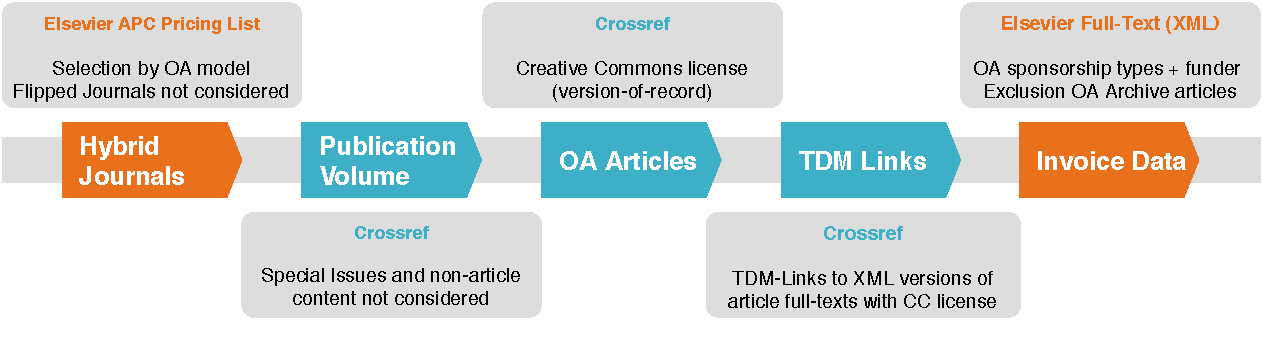
\includegraphics[width=0.95\textwidth]{../figure/els_flow.pdf}

}

\caption{Data Collection Workflow to Obtain Article-Level OA and Invoicing Data.
}\label{fig:workflow}
\end{figure}

First, we identified hybrid journals through an Elsevier APC price list
from May 2020 provided by Matthias (2020). We excluded journals that
transitioned from hybrid to full OA and reverse-flip journals that
flipped from full to hybrid OA (Matthias et al., 2019). Overall, we
identified 1,970 unique hybrid journals that published between 2015 and
2019.

Next, we used an openly available Crossref database snapshot (Crossref,
2020), which contains all Crossref records registered until March 2020,
to calculate the journals' combined article volume for the five-year
period from 2015-2019. We only included articles published in regular
issues aside from supplements containing conference contributions like
meeting abstracts, indicated by non-numeric pagination. We excluded
non-scholarly journal content, such as the table of contents, following
Unpaywall's paratext recognition approach (Unpaywall, n.d.-b), which we
expanded to include patterns indicating corrections. Furthermore, we
categorized the articles by subject according to the All Science Journal
Classification code (ASJC) and added citation indicators from the Scopus
Source Title list (version June 2020) based on the journal they were
published in.

We identified OA articles through CC licenses in Crossref metadata
records (Hendricks et al., 2020) and then downloaded the XML version of
all CC-licensed articles published in a hybrid journal. From the XML
files, we obtained the articles' OA status and invoicing information
(see Table \ref{tab:els_xml}). We determined whether articles were
immediate or delayed OA using the XML node \texttt{openArchiveArticle},
which indicates if an article was made freely available under Elsevier's
Open Archive program, and measured the uptake of hybrid OA. Moreover, we
obtained the invoice channels and recipients of hybrid OA APCs. Using
the \texttt{openaccessSponsorType} node, we distinguished between four
invoice channels, including invoices billed to authors, as part of
publishing agreements with funding bodies (cf. Elsevier (n.d.-a)),
exempted through fee waivers (e.g., in ``cases of genuine need'\,' or
due to society or university sponsorships, cf. Elsevier (n.d.-c)), and
other types not specified by Elsevier. Finally, when hybrid APCs were
invoiced as part of agreements, we identified invoice recipients through
the \texttt{openaccessSponsorName} node. It is worth noting that while
this article focuses on OA articles published in hybrid journals, the
same data is also available for articles published in full OA journals.
Elsevier does not provide the invoiced APC in either case.

\begin{table}[H]
\caption{\label{tab:els_xml}Metadata in Elsevier XML Full-Texts.}
\centering
\begin{tabular}[t]{lp{10cm}}
\toprule
XML node & Description\\
\midrule
\texttt{openaccessArticle} & Was the article open
access? \\
\texttt{openaccessSponsorType} & Invoice channel.\\
\texttt{openaccessSponsorName} & Invoice recipient.\\
\texttt{openArchiveArticle} & Was open access provided through
Elsevier's Open Archive program?\tabularnewline \\
\bottomrule
\end{tabular}
\end{table}

We manually classified invoice recipients based on their institutional
sectors, countries, and primary research areas. Following the OECD's
Frascati Manual (OECD, 2015, p. 91), we coded for four sectors: business
enterprise, government, higher education, and private non-profit. Due to
the low article volume, we combined the business enterprise sector with
invoice recipients Elsevier listed as ``authors'' and ``third-party
sponsor'' into ``Others.'' Moreover, we categorized invoice recipients
according to the countries representing their scope of funding and based
on the following primary research areas health sciences, life sciences,
physical sciences and mathematics, social sciences and humanities, broad
(i.e., multiple research areas), and unknown. Further, we compared
Elsevier's invoicing data with institutional spending data from the Open
APC initiative.

Throughout this mostly automated data gathering and analysis process, we
used tools from the Tidyverse (Wickham et al., 2019) for the R
programming language (R Core Team, 2020). To allow for efficient data
manipulation and retrieval, we imported the Crossref dump to Google
BigQuery, applying the rcrossref (Chamberlain et al., 2020) parsers to
extract relevant metadata fields. We used crminer (Chamberlain, 2020) to
obtain the XML-full texts from Elsevier.

\hypertarget{results}{%
\section*{Results}\label{results}}
\addcontentsline{toc}{section}{Results}

This section first presents the results of our analysis of hybrid OA
uptake in Elsevier's journal portfolio with a view to licensing,
disciplinary differences, and citation impact. Then, we present a
descriptive analysis of Elsevier's invoicing data, highlighting
licensing and disciplinary differences for invoicing channels and
invoice recipients.

\hypertarget{uptake-of-hybrid-open-access}{%
\subsection*{Uptake of Hybrid Open
Access}\label{uptake-of-hybrid-open-access}}
\addcontentsline{toc}{subsection}{Uptake of Hybrid Open Access}

\hypertarget{overview}{%
\subsubsection*{Overview}\label{overview}}
\addcontentsline{toc}{subsubsection}{Overview}

Between 2015 and 2019, 1,755 of 1,970 (89.1\%) hybrid journals published
at least one OA article. Together these journals published 71,643 OA
articles, which represents 3\% of their total article volume
(n=2,422,087). Table \ref{tab:overview} presents findings for each year
and the aggregated five-year period, illustrating moderate growth in
hybrid OA over time. Each year, the number of hybrid journals with at
least one OA article increased, as did the number of immediate OA
articles in these journals, which nearly doubled from 10,672 in 2015 to
19,311 in 2019. However, since the journals' total article output also
grew over time, the relative share of OA articles in hybrid journals
only increased slightly from 2.6\% to 3.7\%.

\begin{table}[H]

\caption{\label{tab:overview}Elsevier Hybrid OA Uptake  2015-2019.}
\centering
\begin{tabular}[t]{lrrrrrr}
\toprule
  & 2015 & 2016 & 2017 & 2018 & 2019 & 2015-19\\
\midrule
\addlinespace[0.3em]
\multicolumn{7}{l}{\textbf{Elsevier Hybrid Journals with ≥ 1 OA article (n)}}\\
\hspace{1em}Total & 1,317.0 & 1,364.0 & 1,401.0 & 1,501.0 & 1,600.0 & 1,755.0\\
\addlinespace[0.3em]
\multicolumn{7}{l}{\textbf{Articles in Elsevier Hybrid Journals with ≥ 1 OA article (n)}}\\
\hspace{1em}Total & 406,701.0 & 422,423.0 & 436,418.0 & 468,952.0 & 518,062.0 & 2,422,087.0\\
\hspace{1em}Avg. & 308.8 & 309.7 & 311.5 & 312.4 & 323.8 & 1,380.1\\
\hspace{1em}SD & 401.1 & 419.6 & 427.5 & 445.6 & 479.9 & 1,937.5\\
\addlinespace[0.3em]
\multicolumn{7}{l}{\textbf{OA Articles in Elsevier Hybrid Journals with ≥ 1 OA article (n)}}\\
\hspace{1em}Total & 10,672.0 & 12,729.0 & 13,361.0 & 15,570.0 & 19,311.0 & 71,643.0\\
\hspace{1em}Mean & 8.1 & 9.3 & 9.5 & 10.4 & 12.1 & 40.8\\
\hspace{1em}SD & 12.9 & 19.7 & 15.6 & 16.2 & 20.1 & 68.9\\
\addlinespace[0.3em]
\multicolumn{7}{l}{\textbf{Share of Elsevier Hybrid Journals with ≥ 1 OA article (\%)}}\\
\hspace{1em}Total & 2.6 & 3.0 & 3.1 & 3.3 & 3.7 & 3.0\\
\hspace{1em}Mean & 3.7 & 4.3 & 4.4 & 4.7 & 5.4 & 3.8\\
\hspace{1em}SD & 4.5 & 5.9 & 5.1 & 4.9 & 5.7 & 4.1\\
\bottomrule
\end{tabular}
\end{table}

Table \ref{tab:overview} also shows that the average OA share per
journal was higher than the overall percentage. To consider these
variations across journals, Figure \ref{fig:boxuptake} illustrates the
range of OA uptake rates as a box-and-whiskers plot by year. The bold
line shows the median OA prevalence across journals, which slightly rose
from 2.4\% in 2015 to 3.7\% in 2019\}. Notably, the upper quartiles and
whiskers stretch farther over the years, which indicates that the range
of uptake among journals with an above-average proportion of OA articles
increased over the years. Nevertheless, the prevalence of hybrid OA
remained relatively low; in 2019, 95\% of Elsevier hybrid journals
published ≤15.6\% of their articles OA.

\begin{figure}[H]

{\centering 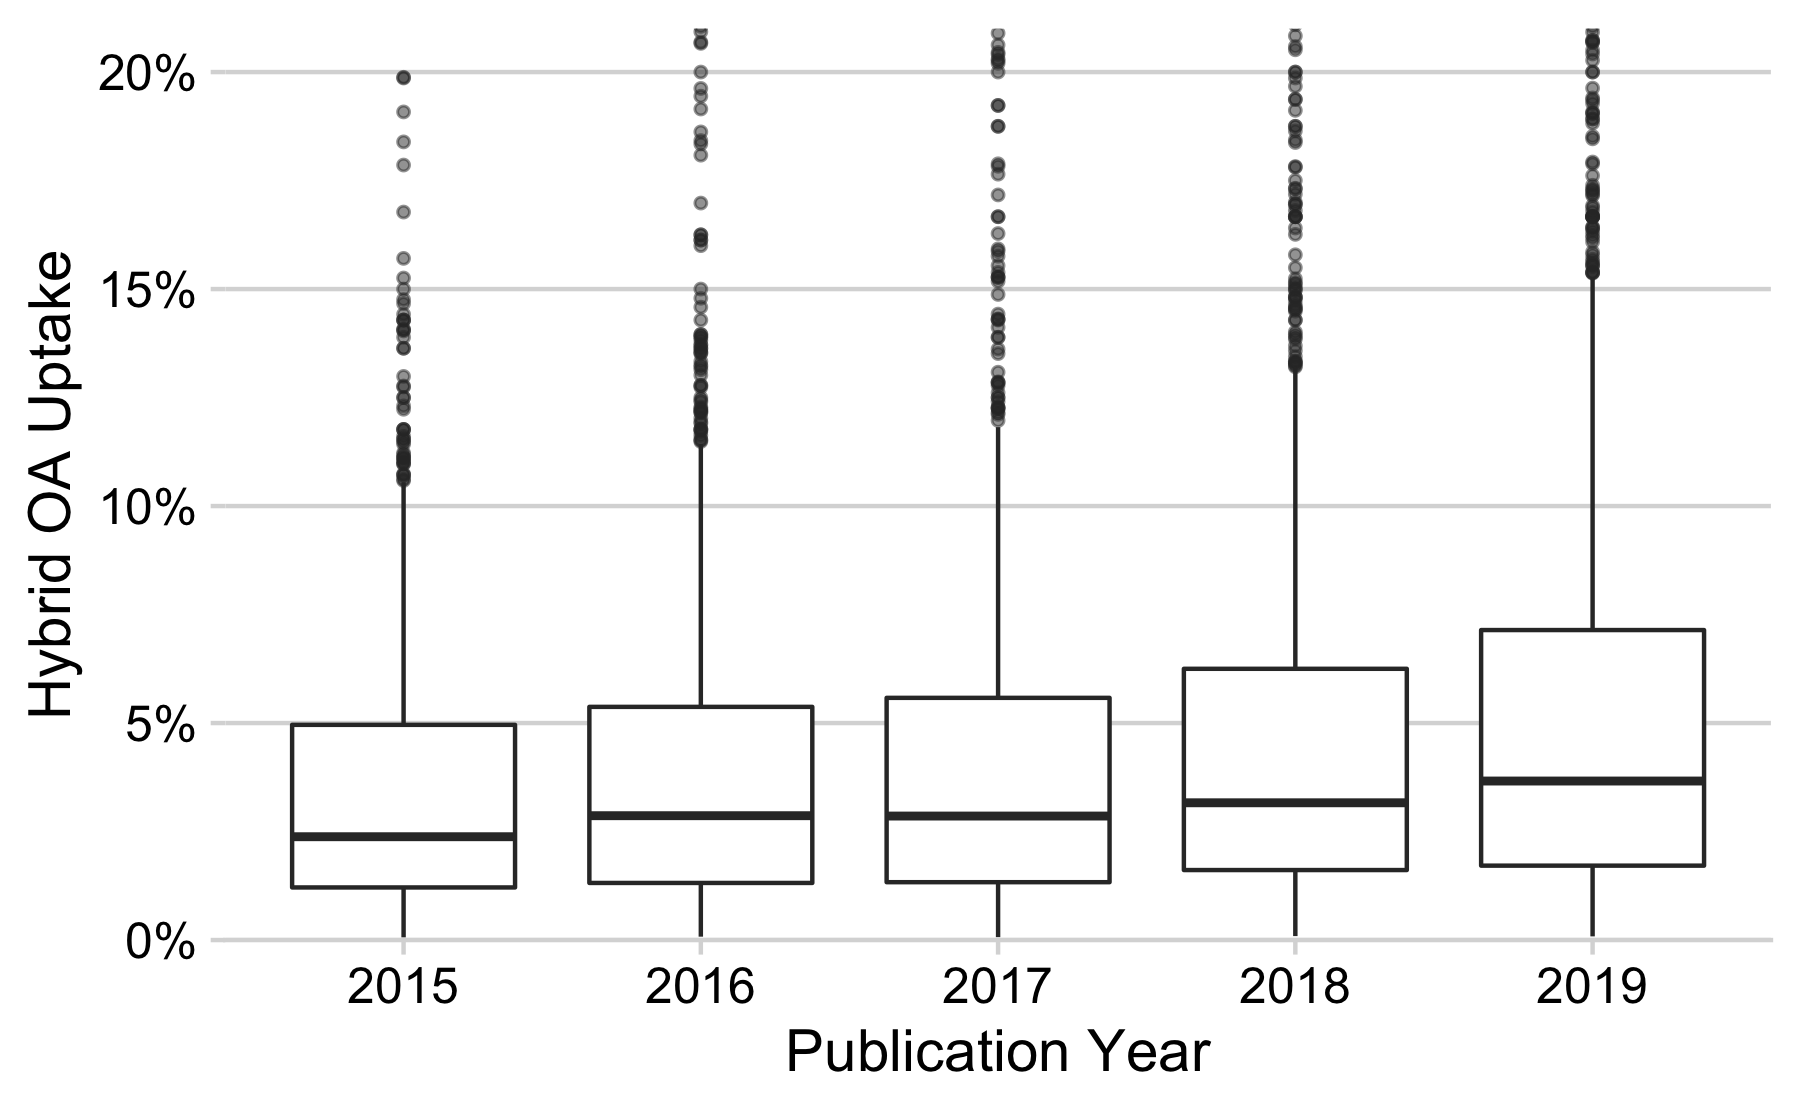
\includegraphics[width=0.7\linewidth,]{manuscript_files/figure-latex/boxuptake-1} 

}

\caption{Open Access Uptake per Elsevier Hybrid Journal (Per Year).}\label{fig:boxuptake}
\end{figure}

During the same period, Elsevier published OA to 328,601 articles in
total (i.e., full, hybrid, and delayed OA combined), representing 12.4\%
of the total article volume (n=2,643,474). Looking at Figure
\ref{fig:oa_volume_fig}, it is apparent that the OA article volume of
hybrid journals (n=71,643; 21.8\%) lagged delayed OA (n=163,643; 49.8\%)
and full OA journals (n=93,315; 28.4\%), which included 817 articles
published in 38 mirror journals.

\begin{figure}[H]

{\centering 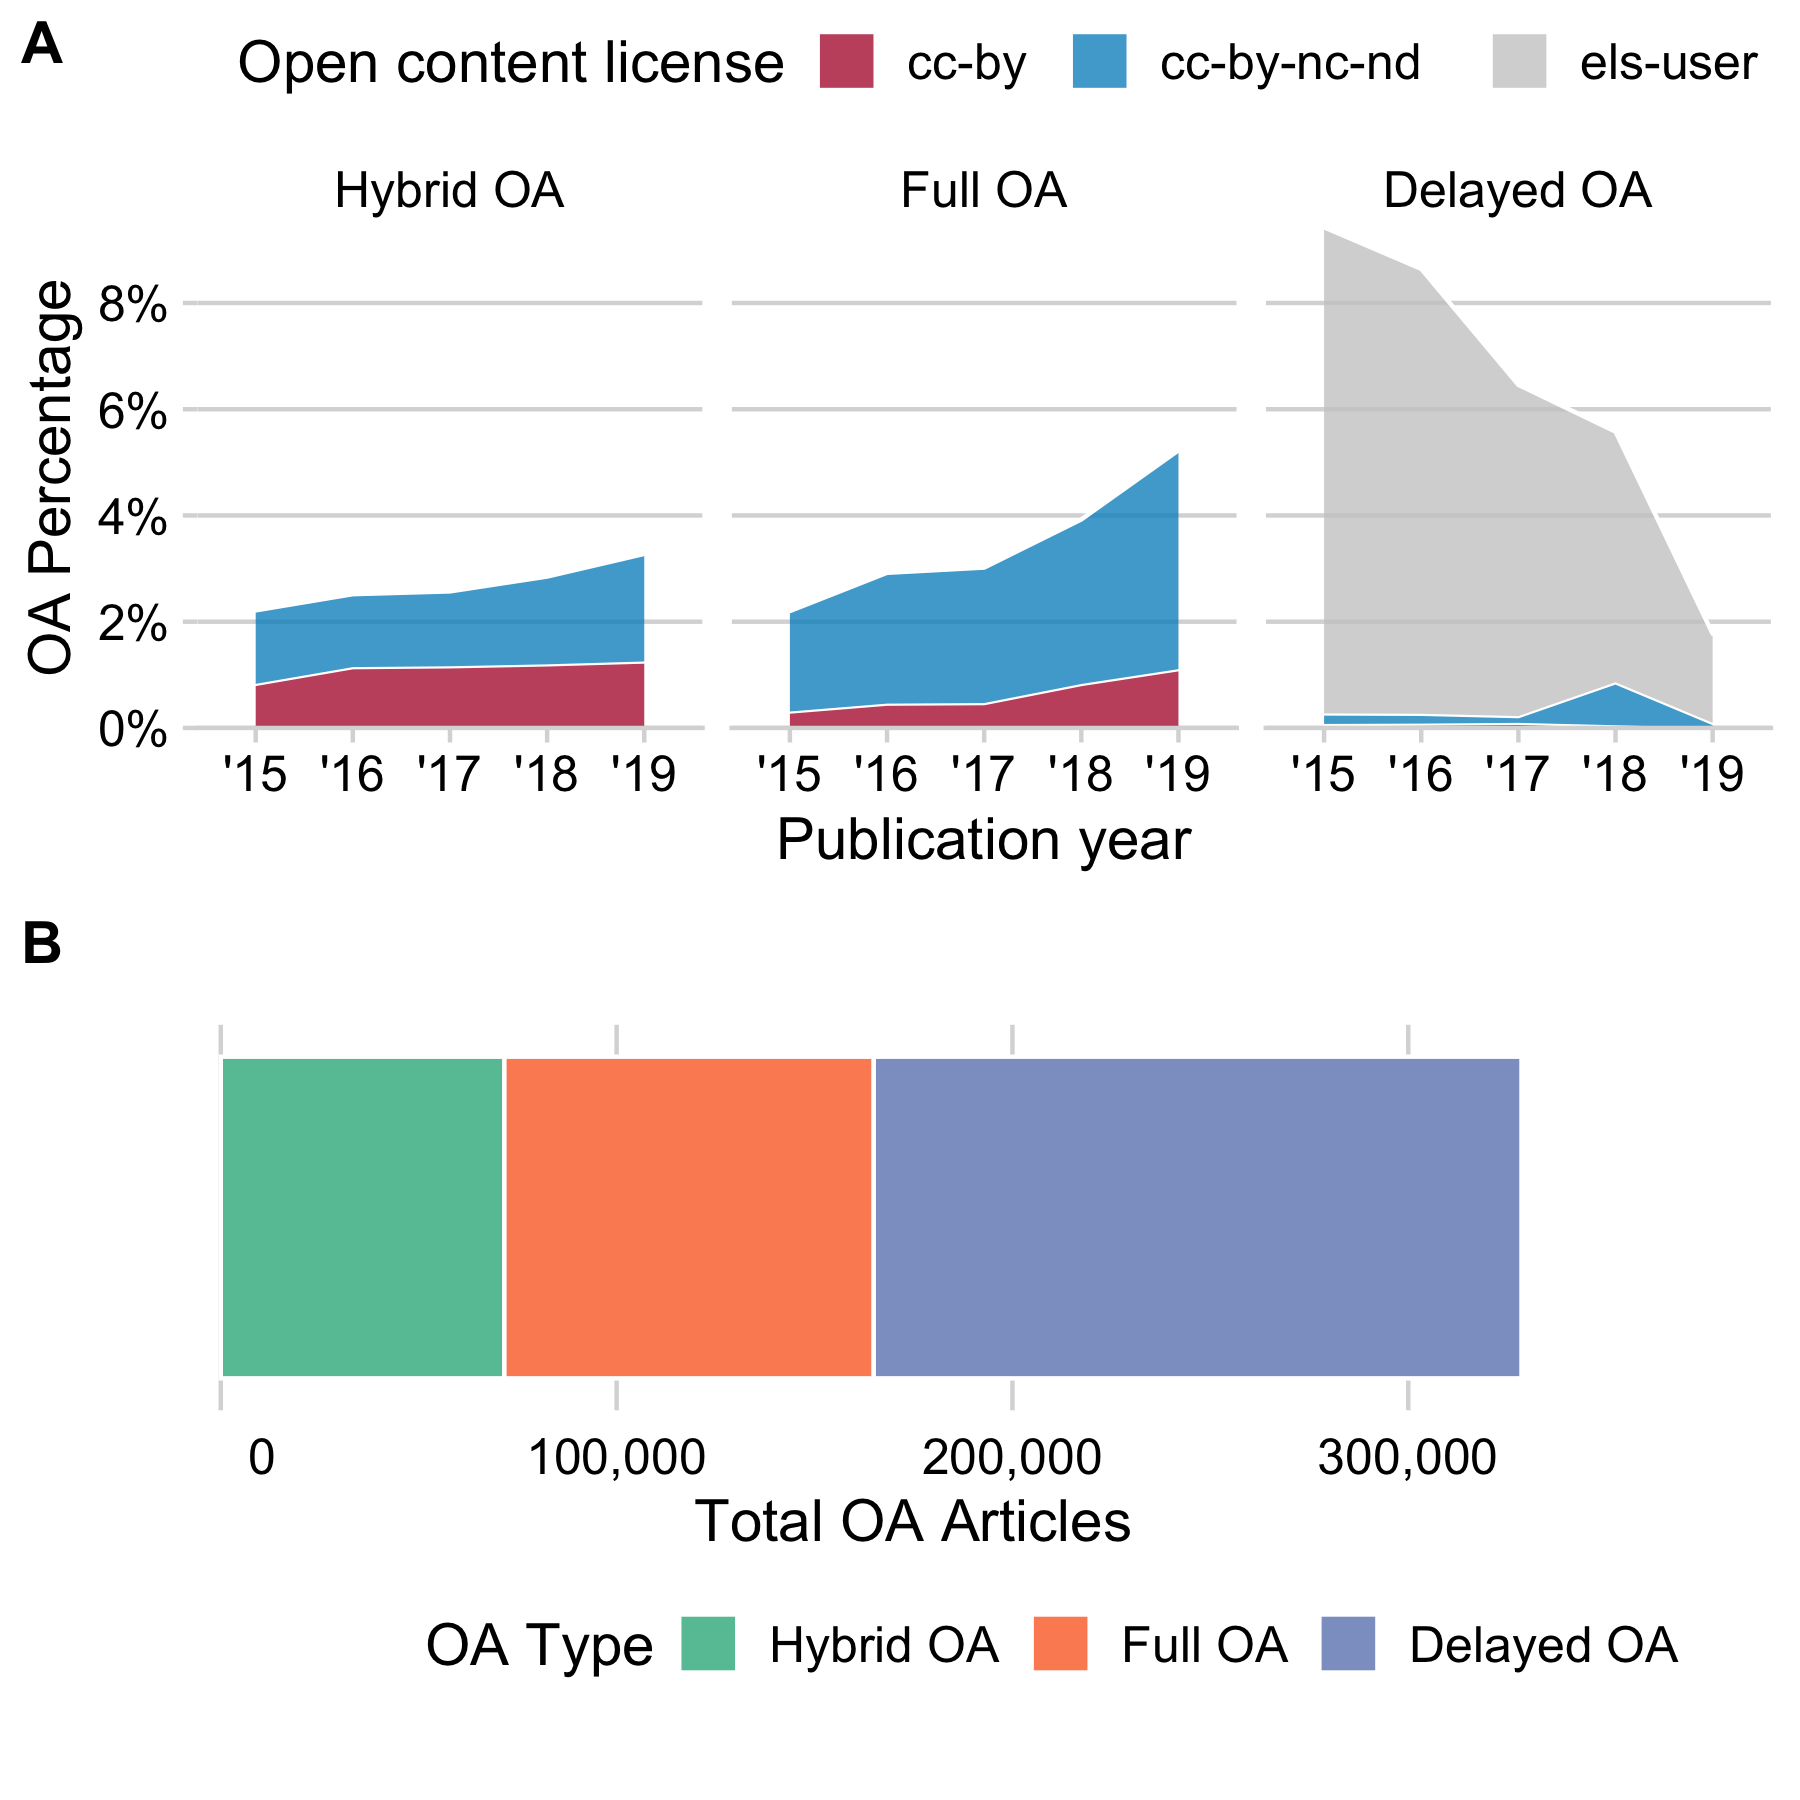
\includegraphics[width=0.7\linewidth,]{/Users/najkojahn/Documents/papers/elsevier_hybrid_invoicing/figure/license_portfolio} 

}

\caption{Elsevier OA Article Volume 2015-2019 by (A) OA Type and (B) Open Content License.}\label{fig:oa_volume_fig}
\end{figure}

\hypertarget{license-prevalence}{%
\subsubsection*{License Prevalence}\label{license-prevalence}}
\addcontentsline{toc}{subsubsection}{License Prevalence}

As far as we observed, OA articles in Elsevier hybrid journals were
published under two possible CC licenses--CC BY or CC BY-NC-ND. CC BY
allows others to distribute, remix, adapt, and build upon the licensed
work, including for commercial purposes, as long as the original author
is credited. In contrast, CC BY-NC-ND is less permissive as it prohibits
commercial reuse and derivatives. In the five-year period from
2015-2019, the proportion of hybrid OA articles published under a CC
BY-NC-ND license marginally increased and maintained a greater share
than that of CC BY (see Figure \ref{fig:oa_volume_fig}-B).
Interestingly, Figure \ref{fig:oa_volume_fig}-B also reveals that hybrid
journals had the highest number and proportion of openly available
articles licensed under CC BY (n=29,752; 41.5\%) compared to full OA
journals (n=17,293; 18.5\%) and Elsevier's delayed OA program (n=1,568;
1\%) . Most delayed OA articles were provided under an Elsevier user
license (Els-User), which prohibits reuse for commercial purposes and
redistribution.

\hypertarget{subject-area-and-field}{%
\subsubsection*{Subject Area and Field}\label{subject-area-and-field}}
\addcontentsline{toc}{subsubsection}{Subject Area and Field}

Next, we present the hybrid OA uptake of different disciplines. Table
\ref{tab:subject_area_table} presents the high-level findings by ASJC
subject area. Between 2015 and 2019, the physical sciences (712 hybrid
journals, 29,584 OA articles) and health sciences (634 hybrid journals,
25,119 OA articles) recorded the most hybrid journals with at least one
OA article. However, the life sciences ((538 hybrid journals, 31,383 OA
articles) published the most hybrid OA articles, while the social
sciences published the least (372 hybrid journals, 11,204 articles). It
is important to note, though, that there is a large overlap between the
journals' subject areas. Therefore, Table \ref{tab:subject_area_table}
also presents fractional counts for hybrid journals and OA articles,
which equally weights counting with respect to the total number of ASJC
subject areas a journal belongs to. Journals with multiple ASJC codes
that are members of the same subject area were counted once. For the
remaining results, we only present the full counting.

\begin{table}

\caption{\label{tab:subject_area_table}Full and Fractional Counting of Subject Areas (2015-2019).}
\centering
\begin{tabular}[t]{lrrrr}
\toprule
\multicolumn{1}{c}{ } & \multicolumn{2}{c}{Full counting} & \multicolumn{2}{c}{Fractional counting} \\
\cmidrule(l{3pt}r{3pt}){2-3} \cmidrule(l{3pt}r{3pt}){4-5}
Subject area & Journals & OA articles & Journals & OA articles\\
\midrule
Health sciences & 634 & 25,119 & 506.6 & 18,415\\
Life sciences & 538 & 31,383 & 368.5 & 21,753\\
Physical sciences & 712 & 29,584 & 584.4 & 23,915\\
Social sciences & 372 & 11,204 & 283.5 & 7,462\\
\bottomrule
\end{tabular}
\end{table}

Figure \ref{fig:oa_sub_uptake} presents the journals' five-year OA
uptake grouped by subject area and field and in comparison to the
overall median (Mdn= 2.5; excluding one journal coded as
multidisciplinary). The box plot reveals some variation between the
subject areas. Notably, with the exception of environmental science and
earth and planetary sciences, journals from the physical sciences show a
lower median proportion of hybrid OA articles, whereas most life
sciences and social sciences journals ranked above average. Figure
\ref{fig:oa_sub_uptake} also shows large variations among the 26 subject
fields, with the highest OA rates in immunology and microbiology
(Mdn=5.1), environmental science (Mdn=4.8), and neuroscience (Mdn=4.3),
whilst chemistry (Mdn=1.4), materials science (Mdn=1.4), and dentistry
(Mdn=0.6) recorded the lowest OA rate.

\begin{figure}[H]

{\centering 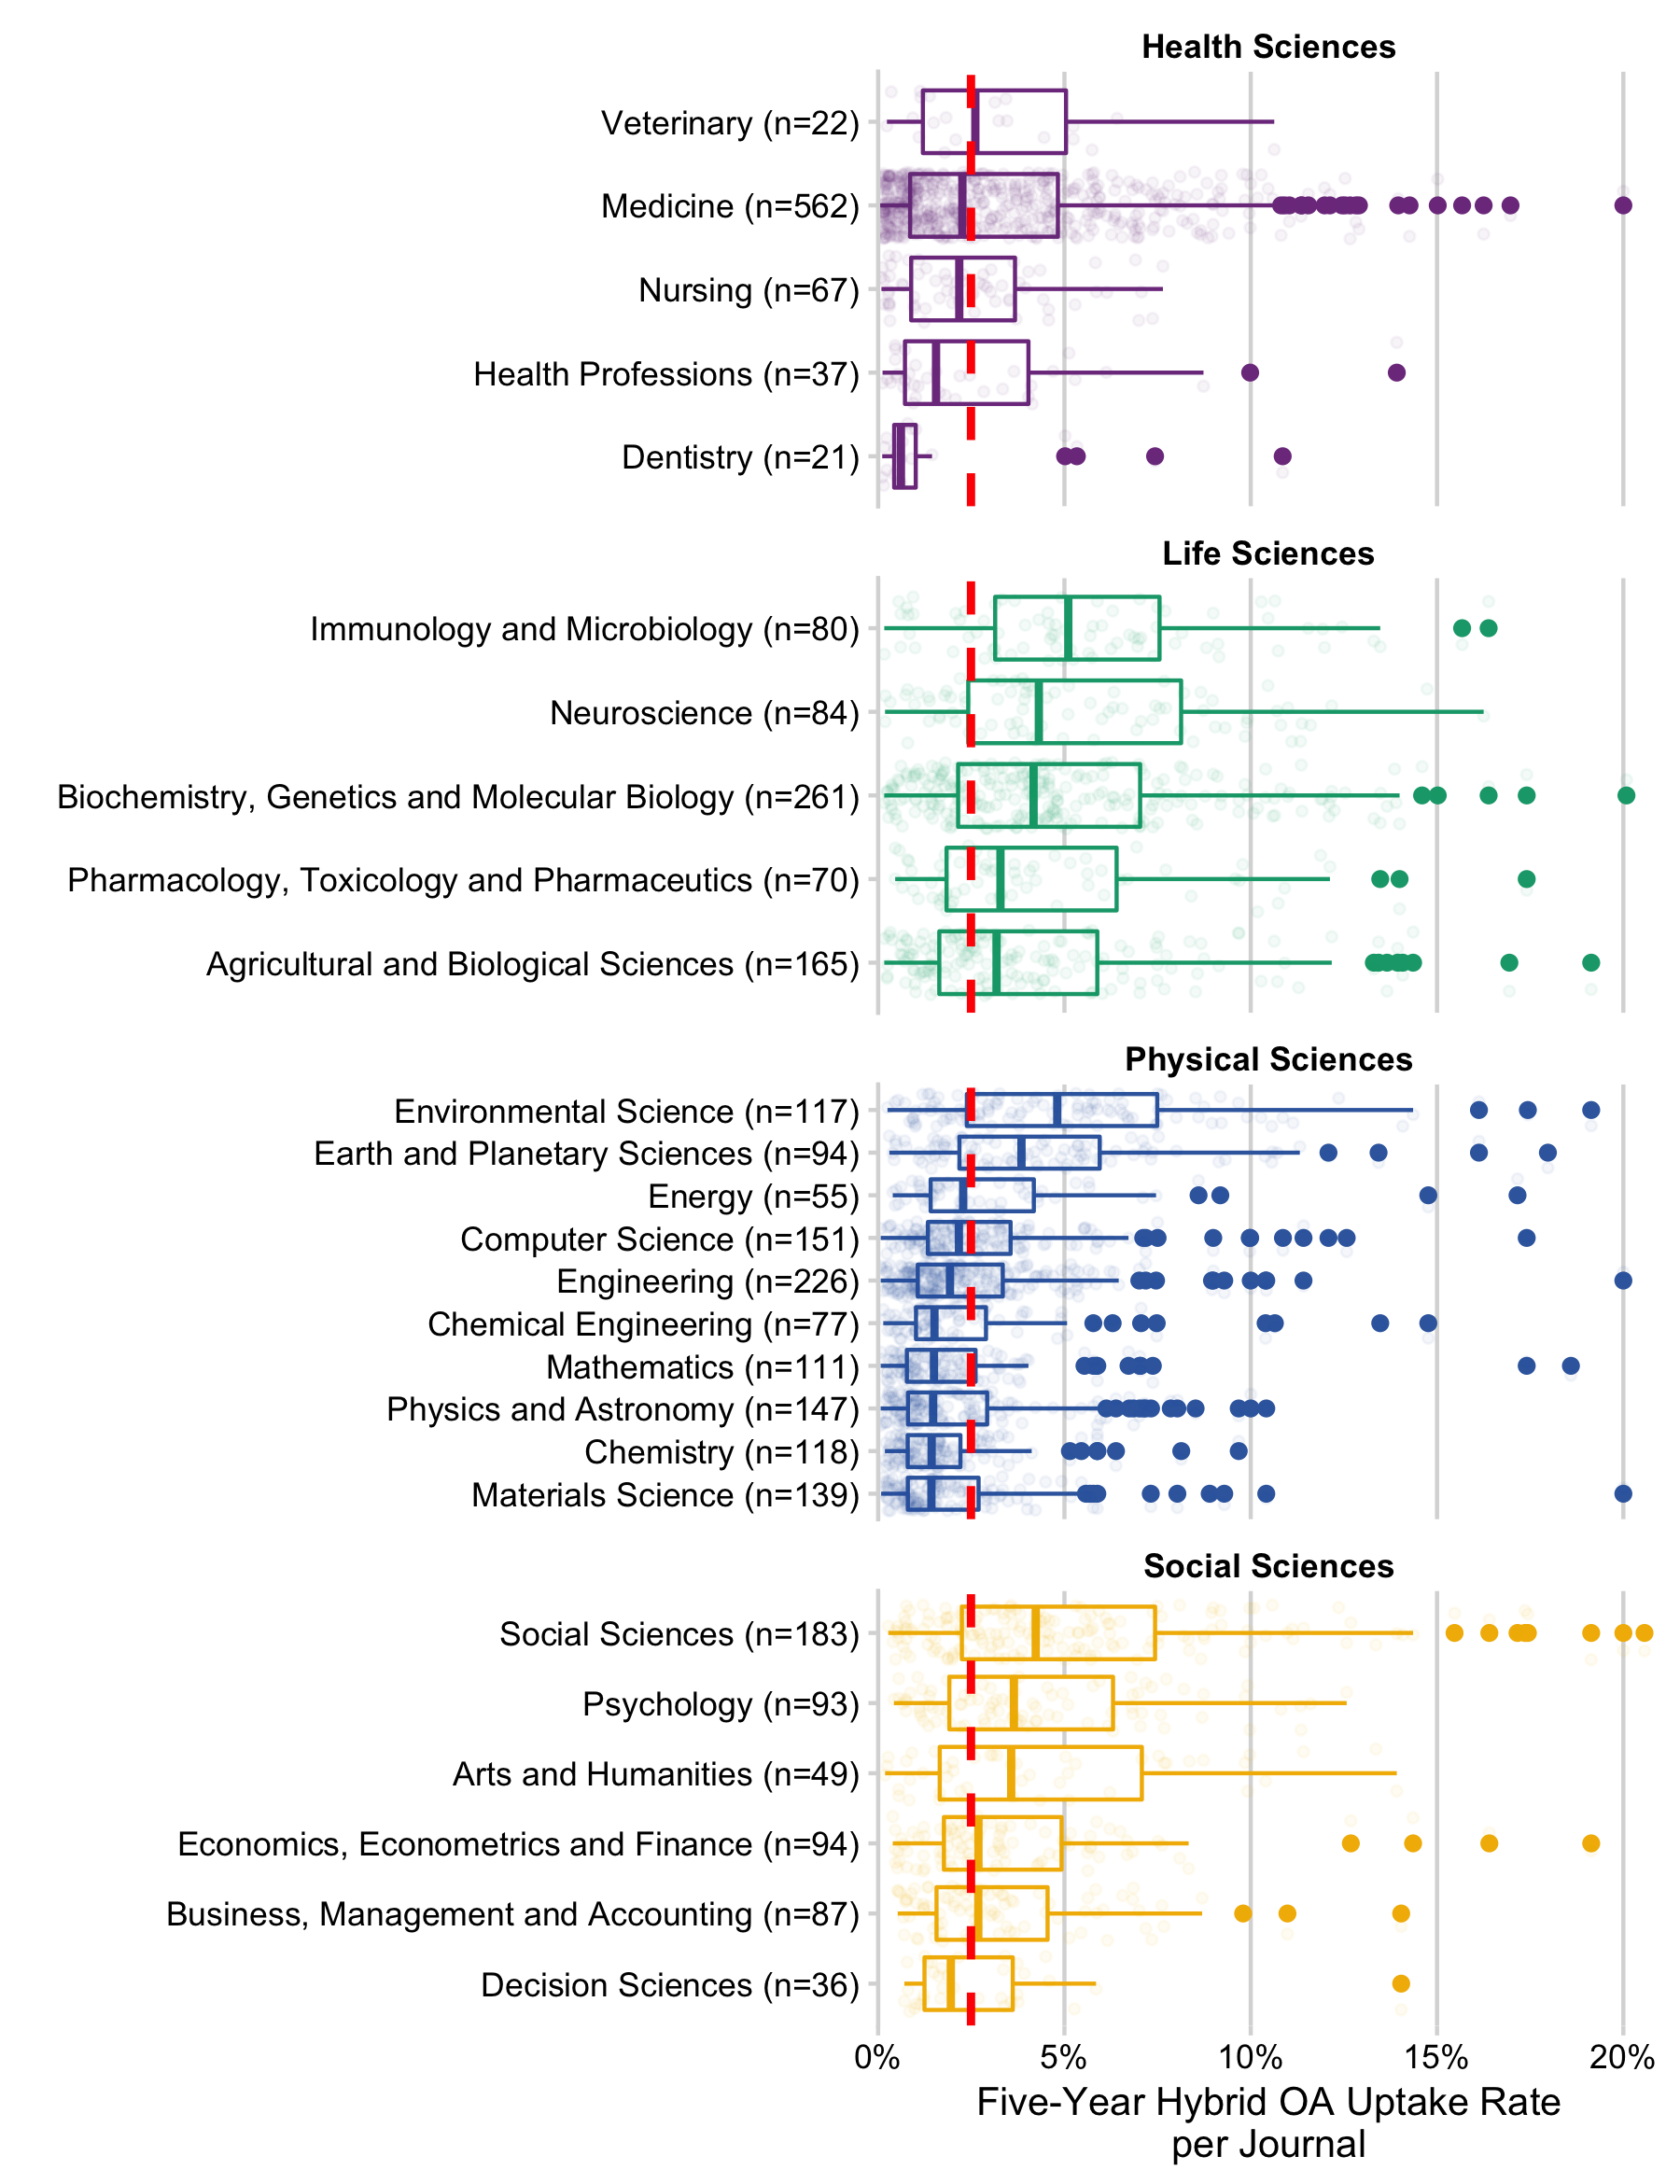
\includegraphics[width=0.9\linewidth,]{manuscript_files/figure-latex/oa_sub_uptake-1} 

}

\caption{OA Uptake in Elsevier Hybrid Journals by Subject Area and Field (2015-2019).}\label{fig:oa_sub_uptake}
\end{figure}

\hypertarget{invoicing-for-hybrid-open-access}{%
\subsection*{Invoicing for Hybrid Open
Access}\label{invoicing-for-hybrid-open-access}}
\addcontentsline{toc}{subsection}{Invoicing for Hybrid Open Access}

\hypertarget{invoice-channels}{%
\subsubsection*{Invoice Channels}\label{invoice-channels}}
\addcontentsline{toc}{subsubsection}{Invoice Channels}

As can be seen from Table \ref{tab:invoicing_overview}, hybrid OA APCs
were most often invoiced to authors (n=41,725; 58.2\%) and to a lesser
extent as part of agreements (n=24,250; 33.8\%). Interestingly, we also
found a small number of cases where hybrid APCs were waived (n=4,345;
6.1\%). A brief note of caution regarding APCs invoiced to the authors
is due here: Although author invoicing was indicated in the
\texttt{openaccessSponsorType} article metadata field used for this
study, this does not necessarily mean that authors paid the APC out of
their own pocket. Rather, this implies that the authors' institution or
funder did not have a central invoicing agreement in place at the time
of publication.

\begin{table}

\caption{\label{tab:invoicing_overview}Invoice Channels for Elsevier Hybrid OA Articles (2015-2019).}
\centering
\begin{tabular}[t]{lrr}
\toprule
Invoicing channel & Hybrid OA articles (n) & Percentage\\
\midrule
Author & 41,725 & 58.2\\
Agreement & 24,250 & 33.8\\
Fee waived & 4,345 & 6.1\\
Other & 1,323 & 1.8\\
\midrule
Total & 71,643 & 100.0\\
\bottomrule
\end{tabular}
\end{table}

Figure \ref{fig:invoiceoverview} illustrates that over the years,
Elsevier has consistently invoiced more authors than funders or academic
consortia (``Agreement''), although both shares increased. In
particular, the proportion of author-invoicing increased from 57\% to
61.2\%, whereas the share of invoicing through agreements slightly
increased from 31.6\% to 32.4\%, respectively. The share of fee-waived
articles also remained relatively stable, but we found different types
of waivers. Around 51.7\% of fee waivers were linked to an OA sponsor,
which indicates that a third party paid the APC. For instance, 853
waivers were linked to the French Académie des Sciences, presumably
covering OA publication in its society journals for affiliated authors.
The remaining 48.3\% of waived articles did not disclose any OA sponsor.
Moreover, Figure \ref{fig:invoiceoverview} compares the invoicing
channels based on open content license variants. When Elsevier invoiced
authors directly, most OA articles in hybrid journals were published
under a non-commercial license (n=32,086; 76.9\%), whereas most articles
billed as part of agreements were licensed under the more permissive CC
BY license (n=18,331; 75.6\%).

\begin{figure}[H]

{\centering 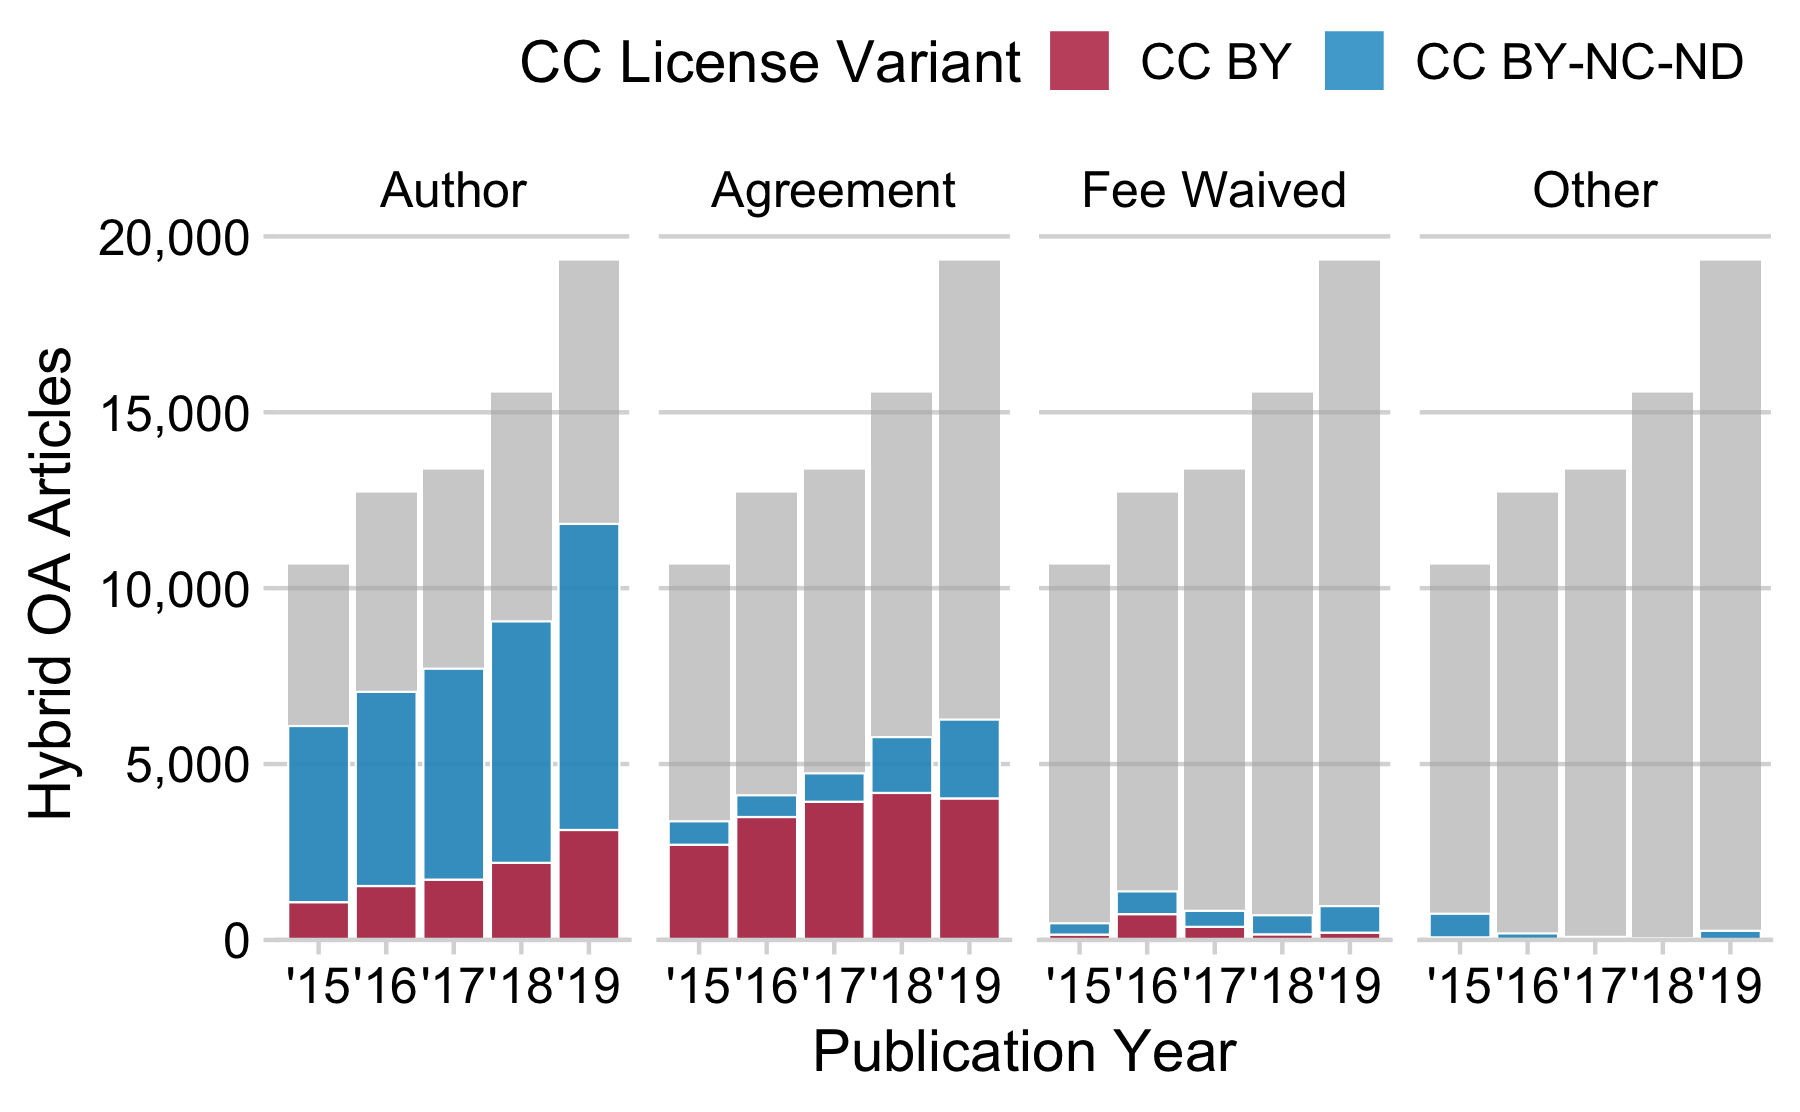
\includegraphics[width=0.7\linewidth,]{manuscript_files/figure-latex/invoiceoverview-1} 

}

\caption{Elsevier Hybrid OA Articles by Invoice Channel and CC License (Per Year).}\label{fig:invoiceoverview}
\end{figure}

We also observed large differences in OA invoicing among subject fields.
Table \ref{tab:invocing_by_subject} shows the number of OA articles by
subject field and invoice channel. For articles in nursing, decision
sciences, and pharmacology, toxicology and pharmaceutics, Elsevier
predominantly invoiced authors, whereas most energy and chemical
engineering articles were invoiced through agreements. Likewise, the
majority of articles in materials science, chemistry and physics and
astronomy were not invoiced to authors but facilitated through
agreements or waived. The large share of waived APCs in physics and
astronomy can be attributed to a single 2015 issue of Nuclear and
Particle Physics Proceedings.

\begin{table}[H]

\caption{\label{tab:invocing_by_subject}Invoice channels by discipline 2015-2019.}
\centering
\resizebox{\linewidth}{!}{
\begin{tabular}[t]{lrrrrr}
\toprule
\multicolumn{2}{c}{ } & \multicolumn{4}{c}{Invoice channel (in \%)} \\
\cmidrule(l{3pt}r{3pt}){3-6}
Subject & OA articles & Author & Agreement & Fee waived & Other\\
\midrule
\addlinespace[0.3em]
\multicolumn{6}{l}{\textbf{Health Sciences}}\\
\hspace{1em}Dentistry & \cellcolor[HTML]{FFFFFF}{288} & \cellcolor[HTML]{EC686E}{68} & \cellcolor[HTML]{FFFAF1}{17} & \cellcolor[HTML]{F89774}{10} & \cellcolor[HTML]{DC3977}{5}\\
\hspace{1em}Health Professions & \cellcolor[HTML]{FFFCF7}{674} & \cellcolor[HTML]{ED6D6E}{67} & \cellcolor[HTML]{FCD898}{24} & \cellcolor[HTML]{FFE8BB}{3} & \cellcolor[HTML]{DC3977}{5}\\
\hspace{1em}Medicine & \cellcolor[HTML]{DC3977}{23623} & \cellcolor[HTML]{F0756E}{65} & \cellcolor[HTML]{FCD092}{25} & \cellcolor[HTML]{FCC98E}{6} & \cellcolor[HTML]{E34F6F}{4}\\
\hspace{1em}Nursing & \cellcolor[HTML]{FFF6E5}{1504} & \cellcolor[HTML]{DC3977}{82} & \cellcolor[HTML]{FFFFFF}{16} & \cellcolor[HTML]{FFF7E8}{1} & \cellcolor[HTML]{FCDE9C}{1}\\
\hspace{1em}Veterinary & \cellcolor[HTML]{FFF2D9}{2091} & \cellcolor[HTML]{F58D72}{61} & \cellcolor[HTML]{FCD092}{25} & \cellcolor[HTML]{F1766E}{13} & \cellcolor[HTML]{FCDE9C}{1}\\
\addlinespace[0.3em]
\multicolumn{6}{l}{\textbf{Life Sciences}}\\
\hspace{1em}Agricultural and Biological Sciences & \cellcolor[HTML]{FCB983}{7956} & \cellcolor[HTML]{F38170}{63} & \cellcolor[HTML]{F9A075}{31} & \cellcolor[HTML]{FCD697}{5} & \cellcolor[HTML]{FCDE9C}{1}\\
\hspace{1em}Biochemistry, Genetics and Molecular Biology & \cellcolor[HTML]{EC686E}{15903} & \cellcolor[HTML]{F89874}{59} & \cellcolor[HTML]{F48671}{35} & \cellcolor[HTML]{FDE1A5}{4} & \cellcolor[HTML]{FAA476}{2}\\
\hspace{1em}Immunology and Microbiology & \cellcolor[HTML]{FCD797}{5542} & \cellcolor[HTML]{F89874}{59} & \cellcolor[HTML]{F58D72}{34} & \cellcolor[HTML]{FCC98E}{6} & \cellcolor[HTML]{FAA476}{2}\\
\hspace{1em}Neuroscience & \cellcolor[HTML]{FCD294}{5906} & \cellcolor[HTML]{FBAA7A}{56} & \cellcolor[HTML]{EC686E}{40} & \cellcolor[HTML]{FFE8BB}{3} & \cellcolor[HTML]{FCDE9C}{1}\\
\hspace{1em}Pharmacology, Toxicology and Pharmaceutics & \cellcolor[HTML]{FEE4AF}{4075} & \cellcolor[HTML]{EA646F}{69} & \cellcolor[HTML]{FCC088}{27} & \cellcolor[HTML]{FFF7E8}{1} & \cellcolor[HTML]{FAA476}{2}\\
\addlinespace[0.3em]
\multicolumn{6}{l}{\textbf{Physical Sciences}}\\
\hspace{1em}Chemical Engineering & \cellcolor[HTML]{FFECC6}{2977} & \cellcolor[HTML]{FFEBC4}{45} & \cellcolor[HTML]{E14971}{47} & \cellcolor[HTML]{FCBC85}{7} & \cellcolor[HTML]{FCDE9C}{1}\\
\hspace{1em}Chemistry & \cellcolor[HTML]{FEE4AF}{4033} & \cellcolor[HTML]{FCE0A1}{48} & \cellcolor[HTML]{E24C70}{46} & \cellcolor[HTML]{FCD697}{5} & \cellcolor[HTML]{FCDE9C}{1}\\
\hspace{1em}Computer Science & \cellcolor[HTML]{FFEAC1}{3185} & \cellcolor[HTML]{F38170}{63} & \cellcolor[HTML]{F27F70}{36} & \cellcolor[HTML]{FFFFFF}{0} & \cellcolor[HTML]{FCDE9C}{1}\\
\hspace{1em}Earth and Planetary Sciences & \cellcolor[HTML]{FDE1A5}{4532} & \cellcolor[HTML]{F89874}{59} & \cellcolor[HTML]{F48671}{35} & \cellcolor[HTML]{FCD697}{5} & \cellcolor[HTML]{FFFFFF}{0}\\
\hspace{1em}Energy & \cellcolor[HTML]{FDE3AA}{4286} & \cellcolor[HTML]{FEE7B8}{46} & \cellcolor[HTML]{DC3977}{52} & \cellcolor[HTML]{FFF7E8}{1} & \cellcolor[HTML]{FCDE9C}{1}\\
\hspace{1em}Engineering & \cellcolor[HTML]{FBB380}{8405} & \cellcolor[HTML]{FCD395}{50} & \cellcolor[HTML]{E24C70}{46} & \cellcolor[HTML]{FFE8BB}{3} & \cellcolor[HTML]{FCDE9C}{1}\\
\hspace{1em}Environmental Science & \cellcolor[HTML]{FBAC7B}{9000} & \cellcolor[HTML]{F99D75}{58} & \cellcolor[HTML]{EF726E}{38} & \cellcolor[HTML]{FFE8BB}{3} & \cellcolor[HTML]{FCDE9C}{1}\\
\hspace{1em}Materials Science & \cellcolor[HTML]{FCDF9E}{4838} & \cellcolor[HTML]{FCDA99}{49} & \cellcolor[HTML]{E14971}{47} & \cellcolor[HTML]{FDE1A5}{4} & \cellcolor[HTML]{FFFFFF}{0}\\
\hspace{1em}Mathematics & \cellcolor[HTML]{FFF2D8}{2105} & \cellcolor[HTML]{FCBF87}{53} & \cellcolor[HTML]{EF726E}{38} & \cellcolor[HTML]{FBAF7D}{8} & \cellcolor[HTML]{FFFFFF}{0}\\
\hspace{1em}Physics and Astronomy & \cellcolor[HTML]{FCD394}{5859} & \cellcolor[HTML]{FFFFFF}{40} & \cellcolor[HTML]{EF726E}{38} & \cellcolor[HTML]{DC3977}{22} & \cellcolor[HTML]{FFFFFF}{0}\\
\addlinespace[0.3em]
\multicolumn{6}{l}{\textbf{Social Sciences}}\\
\hspace{1em}Arts and Humanities & \cellcolor[HTML]{FFF6E4}{1565} & \cellcolor[HTML]{FCB882}{54} & \cellcolor[HTML]{E4536F}{44} & \cellcolor[HTML]{FFF7E8}{1} & \cellcolor[HTML]{FFFFFF}{0}\\
\hspace{1em}Business, Management and Accounting & \cellcolor[HTML]{FFF4E0}{1751} & \cellcolor[HTML]{EC686E}{68} & \cellcolor[HTML]{FBAF7D}{29} & \cellcolor[HTML]{FFF0D2}{2} & \cellcolor[HTML]{FCDE9C}{1}\\
\hspace{1em}Decision Sciences & \cellcolor[HTML]{FFFBF4}{785} & \cellcolor[HTML]{E6576F}{72} & \cellcolor[HTML]{FCC088}{27} & \cellcolor[HTML]{FFFFFF}{0} & \cellcolor[HTML]{FCDE9C}{1}\\
\hspace{1em}Economics, Econometrics and Finance & \cellcolor[HTML]{FFF2D9}{2071} & \cellcolor[HTML]{F48771}{62} & \cellcolor[HTML]{F79373}{33} & \cellcolor[HTML]{FCD697}{5} & \cellcolor[HTML]{FFFFFF}{0}\\
\hspace{1em}Psychology & \cellcolor[HTML]{FFEBC3}{3087} & \cellcolor[HTML]{FAA376}{57} & \cellcolor[HTML]{EC686E}{40} & \cellcolor[HTML]{FFF0D2}{2} & \cellcolor[HTML]{FCDE9C}{1}\\
\hspace{1em}Social Sciences & \cellcolor[HTML]{FCCD91}{6306} & \cellcolor[HTML]{F79273}{60} & \cellcolor[HTML]{F27F70}{36} & \cellcolor[HTML]{FFE8BB}{3} & \cellcolor[HTML]{FFFFFF}{0}\\
\bottomrule
\end{tabular}}
\end{table}

\hypertarget{invoice-recipients}{%
\subsubsection*{Invoice Recipients}\label{invoice-recipients}}
\addcontentsline{toc}{subsubsection}{Invoice Recipients}

Elsevier's data offer more insight into invoicing. Overall, we
identified 63 academic institutions and funders that received invoices
as part of publishing agreements. By a large margin, most invoices were
issued to UK-based research funders and institutions (n=14,344; 59.2\%),
followed by the Netherlands (n=2,835; 11.7\%) and the European Union
(n=1,990; 8.2\%; EU), which in the context of this paper refers to
institutions established by the European Commission, and not the
individual member states. Invoicing data comprises two EU institutions,
the research funder European Research Council and the health agency
European Center for Disease Prevention and Control (ECDS). Figure
\ref{fig:invoice_sponsor_country} presents the geographical distribution
by license prevalence, highlighting the dominance of CC BY licensed
articles invoiced to institutions in the UK, the United States (US),
and, to a much lesser extent, the Netherlands. In contrast, most
articles invoiced to institutions from Norway or representing the EU
were published under a non-commercial license.

\begin{figure}[H]

{\centering 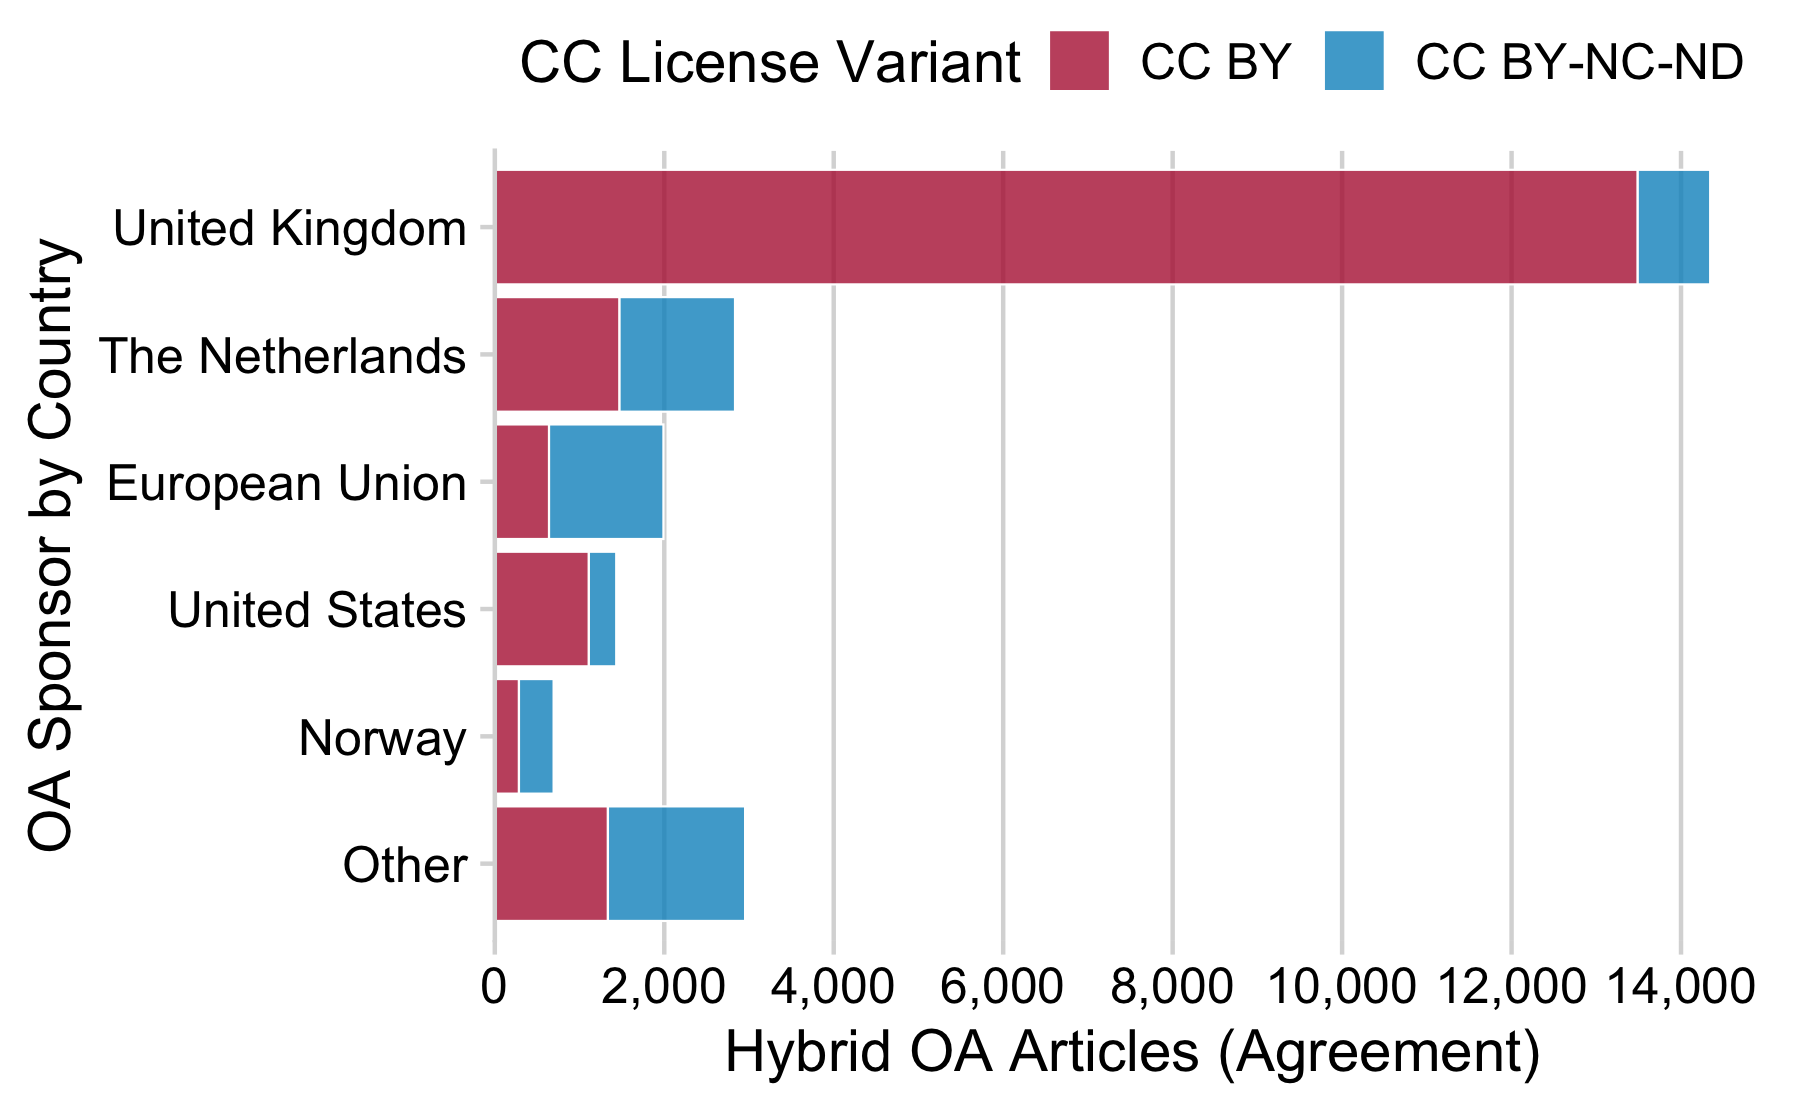
\includegraphics[width=0.7\linewidth,]{manuscript_files/figure-latex/invoice_sponsor_country-1} 

}

\caption{Centrally Invoiced Elsevier Hybrid OA Articles by Country and CC License (2015-2019).}\label{fig:invoice_sponsor_country}
\end{figure}

Figure \ref{fig:sponsor_sector} shows the yearly distribution of
centrally invoiced articles by year and institutional sector. While
UK-based OA invoices were mainly addressed to discipline-specific
governmental and non-profit research funders, invoices to the
Netherlands and Norway were issued to national academic consortia
representing the higher education sector. In 2019, Elsevier also
launched similar agreements in countries with lower publication output
including Hungary and Poland. We found that invoice recipients from the
UK and the US mainly represented discipline-specific funders, while
invoice recipients from other countries focused on a broad variety of
disciplines.

\begin{figure}[H]

{\centering 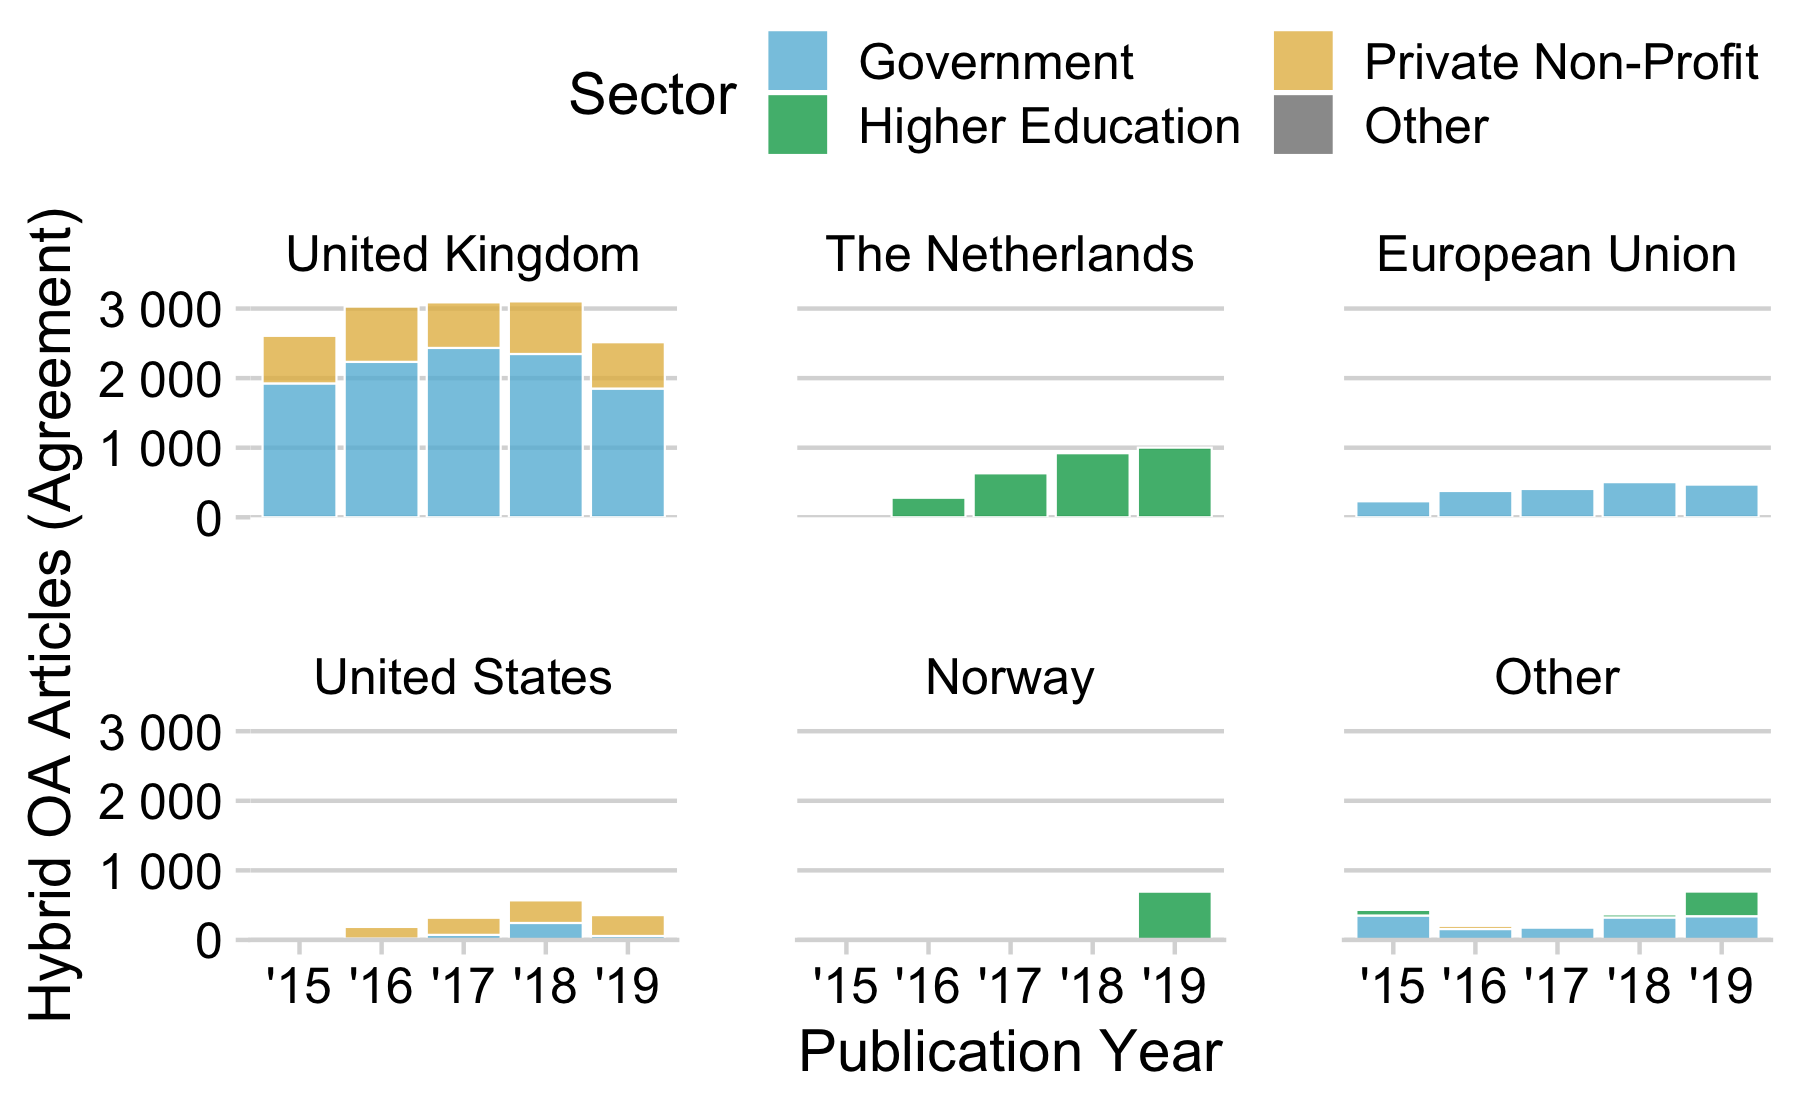
\includegraphics[width=0.7\linewidth,]{manuscript_files/figure-latex/sponsor_sector-1} 

}

\caption{Centrally Invoiced Elsevier Hybrid OA Articles by Country and Sector (Per Year).}\label{fig:sponsor_sector}
\end{figure}

Table \ref{tab:sponsor_top_10} presents the top ten of 63 sponsoring
bodies in our sample. Together, they accounted for around 80\% of
centrally invoiced APCs. The table also highlights the number of
distinct journals and the share of CC BY licensed articles. Notably,
UK-based research funders and the US-based Bill and Melinda Gates
Foundation mainly received invoices for CC BY licensed articles. In
contrast, articles invoiced to VSNU, the European Research Council, and
Norway Institutes had a much lower proportion of CC BY.

\begin{table}

\caption{\label{tab:sponsor_top_10}Elsevier Hybrid OA Invoice Recipients  (2015-2019).}
\centering
\resizebox{\linewidth}{!}{
\begin{tabular}[t]{lrrrrr}
\toprule
\multicolumn{4}{c}{ } & \multicolumn{2}{c}{Compliance (in \%)} \\
\cmidrule(l{3pt}r{3pt}){5-6}
Hybrid OA sponsors & Journals & Articles & \% & CC BY & OAPC\\
\midrule
Engineering and Physical Sciences Research Council & 619 & 4663 & 19 & \cellcolor[HTML]{DE3E75}{97} & \cellcolor[HTML]{E34E6F}{55}\\
VSNU & 357 & 2835 & 12 & \cellcolor[HTML]{FCC38A}{52} & \cellcolor[HTML]{FFFFFF}{0}\\
Wellcome Trust & 448 & 2506 & 10 & \cellcolor[HTML]{DD3D76}{98} & \cellcolor[HTML]{DD3D76}{66}\\
European Research Council & 541 & 1986 & 8 & \cellcolor[HTML]{FFFFFF}{32} & \cellcolor[HTML]{FFE9BD}{9}\\
Medical Research Council & 384 & 1922 & 8 & \cellcolor[HTML]{DF4274}{95} & \cellcolor[HTML]{E6596F}{51}\\
Natural Environment Research Council & 203 & 1357 & 6 & \cellcolor[HTML]{DE3E75}{97} & \cellcolor[HTML]{EC696E}{45}\\
Biotechnology and Biological Sciences Research Council & 309 & 1169 & 5 & \cellcolor[HTML]{E04573}{93} & \cellcolor[HTML]{F0736E}{41}\\
Bill and Melinda Gates Foundation & 254 & 1030 & 4 & \cellcolor[HTML]{DC3977}{100} & \cellcolor[HTML]{DC3977}{68}\\
Economic and Social Research Council & 245 & 922 & 4 & \cellcolor[HTML]{DE4075}{96} & \cellcolor[HTML]{E9616F}{48}\\
Norway Institutes & 374 & 694 & 3 & \cellcolor[HTML]{FFE9BD}{41} & \cellcolor[HTML]{FFFFFF}{0}\\
Other & 1012 & 5166 & 21 & \cellcolor[HTML]{FCBA84}{54} & \cellcolor[HTML]{FCBF87}{21}\\
\midrule
All & 1423 & 24250 & 100 & \cellcolor[HTML]{ED6C6E}{76} & \cellcolor[HTML]{F48671}{36}\\
\midrule
\bottomrule
\end{tabular}}
\end{table}

The table also highlights the proportion of APC funding publicly
disclosed through the Open APC initiative, showing higher disclosure
rates for funders with a large CC BY share. On the other hand, APCs that
were invoiced as part of transformative agreements were not publicly
shared.

\hypertarget{discussion}{%
\section{Discussion}\label{discussion}}

From 2015-2019, Elsevier recorded growth in the uptake of hybrid OA: The
number of hybrid OA articles published per year doubled, the number of
hybrid journals with at least one OA article grew by 21\%, and the share
of hybrid OA articles relative to closed-accessed articles in these
journals increased from 2.6\% to 3.7\%. As Laakso \& Björk (2016), we
observed disciplinary differences. In particular, we found the highest
count of hybrid OA articles in physical sciences journals (see Table
\ref{tab:subject_area_table}). This was followed by the life sciences
and health sciences, whereas the social sciences had the lowest count.
This order mostly reflects the disciplines' overall publication output.
According to the Open Science Monitor (European Commission, 2019), the
physical sciences publish the most articles, followed by the health
sciences, life sciences, and social sciences.

Disciplinary differences in hybrid OA prevalence become more meaningful
when considering the relative share of OA articles to closed-access
articles. In line with previous research, we found that Elsevier
journals from the life sciences and social sciences (Jubb et al., 2017;
Kramer \& Bosman, 2018; Laakso \& Björk, 2016) recorded greater than
typical hybrid OA uptake, whereas physical sciences journals generally
had a lower than typical uptake (Kramer \& Bosman, 2018; Laakso \&
Björk, 2016; Martín-Martín et al., 2018). In a systematic review of
disciplinary OA publishing patterns, Severin et al. (2020) highlighted
the importance of socio-cultural and technological factors in shaping
publishing cultures and practices. For instance, since many branches of
the physical sciences have established self-archiving practices Laakso
\& Björk (2016), researchers can provide OA through repositories and
might perceive much less of a need for hybrid OA. In contrast, hybrid OA
in the life sciences could be enabled through project-based funding
structures as they allow for easy integration of publishing costs
Severin et al. (2020). On the other hand, the high hybrid OA uptake that
we observed among the social sciences could point to the influential
role of OA policies and invoicing agreements (Huang et al., 2020;
Larivière \& Sugimoto, 2018). While these aspects are important drivers
of both full and hybrid OA, faculty members generally prioritize journal
prestige and the journal impact factor (Niles et al., 2020) in
publishing decisions, which, in combination with the availability of OA
funding, might encourage publishing hybrid OA (Graaf et al., 2017).

Our invoicing data analysis found that most APCs were invoiced to the
author (n=41,725; 58.2\%). However, it is important to emphasize
although Elsevier's metadata classifies the sponsor type as
``author'\,', this does not necessarily mean that authors paid for APCs
themselves but rather that APCs were not invoiced through publishing
agreements. It is possible that these APCs were covered through
institutional funds or research grants. This would align with a recent
Springer Nature survey that found hybrid OA was predominantly supported
through institutional and funder sources (71\%), followed by OA
agreements (34\%), while only 6\% were paid from personal funds or
savings (Monaghan et al., 2020).

Further, we observed notable differences in licensing. Most hybrid OA
articles invoiced to author were licensed under the more restrictive CC
BY-NC-ND license. Previous research, while lacking dedicated studies on
license selection, suggests that authors tend to select more restrictive
license variants when given a choice (Fraser et al., 2021; Noorden,
2013; Rowley et al., 2017). On the other hand, we found when hybrid OA
was invoiced through agreements, most articles were licensed under the
more liberal CC BY license. As several funding bodies mandate CC BY
licenses, including the UK research funders that account for 62\% of our
``agreement'' subsample, this result is perhaps not surprising but
suggests the effectiveness of such agreements.

Based on our findings, around a third of the articles were invoiced
through OA agreements (e.g., research funders, national library
consortia). The predominance of UK funding bodies in this subsample
reiterates reports from previous studies that the UK's OA profile
differs markedly from other countries (cf. Jubb et al. (2015); Jubb et
al. (2017)), pointing to the impact of science policy. To promote OA,
the UK implemented centralized APC funding and embraced hybrid OA as a
transition model. Within five years of the publication of the Finch
Report in 2012, the UK recorded an 18\% increase in immediate OA,
coupled with a rise in hybrid OA from 2.7\% in 2012 to 15.4\% of all
articles in 2016 (Jubb et al., 2017), which can be attributed to the
availability of funding from RCUK. Indeed, RCUK block grants have been
the largest single source of APC funds in the UK---the Wellcome Trust,
and more recently transformative agreements (Jubb et al., 2017; Tickel,
2018). However, since then publishing expenditures of UK universities
have been rising rapidly (Jubb et al., 2017), so that several
universities stopped supporting hybrid OA in late 2018-2019 (University
of Birmingham, n.d.; Walker, 2019). This development might explain the
slight decrease in hybrid articles invoiced to the UK our data showed
around that time (see Figure \ref{fig:sponsor_sector}).

Through this study we demonstrated the utility and benefits of
publisher-provided metadata about hybrid OA invoicing and highlighted
the need for extending these to include comprehensive information about
licensing and APC waivers. Metadata guidance should also consider the
substantial amount of delayed OA content, which needs to be
distinguished from hybrid OA. Hence, our study substantiates the
recommendations from the ESAC Initiative that seek to increase
efficiency and transparency through improved invoicing and reporting
processes and metadata about OA funding (Geschuhn \& Stone, 2017;
Marques et al., 2019).

While this study advances our knowledge about hybrid OA uptake and
invoicing, the limitations leave room for future research. We focused on
only one publisher, which limits the generalizability of our findings
because Elsevier's journal portfolio, mix of business models, pricing,
and promotion of various options cannot be assumed to be representative
of scholarly journal publishing in general. Relatedly, our study is
limited to articles published in hybrid OA journals and, hence, is not
representative of invoices for articles in full OA journals. To develop
a full picture of OA invoicing, the methodology presented in this paper
can be used for future studies in this direction. Further, although
Elsevier's invoicing data improves transparency, it seems likely that
not all actual OA funding bodies are disclosed. For instance, most
articles were invoiced to authors, but it remains unclear if the APCs
were paid by the authors themselves or through institutional OA funds or
research grants. Research into this topic would improve our
understanding of OA funding outside of publishing agreements. Moreover,
our study demonstrates that comprehensive mapping of the financial flows
of OA publishing requires complex, in-depth country-specific analyses.
Such studies would ideally draw on various data sources to consider
research funders, the consortia landscape, OA policies, and publishing
agreements Future research could analyze funder policies in combination
with institutional agreements (including which journals are covered by
the agreements) and hybrid OA invoicing metadata to provide more insight
into publishing patterns and CC licence choice. A further avenue of
research would be dedicated studies on the strengths and weaknesses of
data provided by publishers and the Open APC initiative, and consider an
integrative approach that combines both datastreams to reap the benefits
of each while mitigating their individual drawbacks.

The policy implications and the underlying data of this study present
opportunities for actors in the scholarly publishing landscape to rely
less on assumptions and secondary data, and instead establish a direct
connection between the publication output and the related financial
information. This could increase accountability in spending public and
charitable funds, and improve OA cost monitoring through enhanced
transparency, precision, and timeliness. Analyses like we have presented
here can inform library consortia in negotiations through better
understanding their publisher-specific OA output, determining the amount
of delayed OA content, and facilitating comparative analyses across
different consortia. The study could also inform research funders and
research institutions about license selection implications if there is
not any strict policy in place. This study provides a snapshot of hybrid
OA for Elsevier, the largest journal publisher, prior to the impact of
the implementation of Plan S, an initiative to accelerate the transition
to OA that will no longer support hybrid OA (cOAlition S, n.d.). While
many Plan S signatories have already had strong OA policies, this
harmonized approach is likely to affect publishing decisions of funded
authors, the licencing of their articles, and the offerings and pricing
of publishers at a larger scale than before. Because the new
requirements apply to research funded from 2021 onward, a comparative
study on articles invoiced to Plan S signatories would be a fruitful
endeavor. Plan S does not fund hybrid OA publication unless the host
journal is explicitly committed to convert to full OA, however, with the
growth of national and institutional agreements that enable affiliated
authors to publish hybrid OA, such restrictions will influence
researchers differently. Invoicing data as used for this study can be
useful in exploring later on, by looking at research funding statements
and invoicing channels in relation to each other.

\hypertarget{conclusion}{%
\section{Conclusion}\label{conclusion}}

The primary aim of this empirical study was to investigate Elsevier's
hybrid OA publishing from 2015-2019 to better understand the volume and
invoicing of hybrid OA and to present a novel, data-driven approach for
such analyses. Our results indicate that although the number of hybrid
OA articles has increased over time, its uptake has remained low.
Notably, hybrid APCs were most often invoiced directly to the authors,
followed by agreements, where only a few funding bodies were the primary
drivers of hybrid OA. Finally, our findings highlight that
publisher-provided metadata about the invoicing channels of (hybrid) OA
can facilitate research into and increase the understanding of the
financial flows of OA publishing.

Since the beginning, hybrid OA has been a challenging subject to study
due to the lack of standardized ways publishers flag such content and
APC funding data being limited self-reported data, surveys, and other
secondary sources. This study presented a novel approach to studying APC
invoicing that is based on publicly available publisher-provided
metadata, which can be used on on its own or in combination with other
public data sources to gain more detailed and comprehensive insights
into hybrid OA uptake and invoicing. If more publishers reported OA
invoicing on the article level and in a machine-readable format, this
would increase transparency and improve monitoring of the scholarly
journal landscape over time. As hybrid OA has become a central element
of OA policies of research funders and libraries, consumer organizations
could require that invoicing information is added to the article-level
metadata. As long as publishers do not provide this data in a structured
and comprehensive format, they prevent benchmarking prices and therefore
hinder competition.

From recent science policy developments in Europe it appears that Big
Deals have gained support and remain firmly in place in the form of
transformative agreements. Moreover, such agreements seem to become an
increasingly dominant feature of scholarly publishing as indicated by
the number of contracts that Elsevier and other publishers have
successfully negotiated and secured since we conducted the analyses
presented here.\footnote{See, for instance, the announcements from the
  University of California:
  \url{https://www.universityofcalifornia.edu/news/uc-s-deal-elsevier-what-it-took-what-it-means-why-it-matters}
  and the Danish National Licensing Consortium:
  \url{https://www.kb.dk/en/about-us/licensing/national-licensing-consortium/elsevier-agreement-2021-24}}
Through this study we can affirm that hybrid OA is complex as the
financial flows involve research funders, libraries, consortia, and
authors. However, it is on publishers to increase the transparency of OA
publishing, including hybrid OA and transformative agreements, by
providing instantaneous open data about OA uptake and invoicing.

\hypertarget{data-availability}{%
\section{Data Availability}\label{data-availability}}

The source code data analysis is available on GitHub:

\url{https://github.com/njahn82/elsevier_hybrid_invoicing}

\hypertarget{references}{%
\section*{References}\label{references}}
\addcontentsline{toc}{section}{References}

\hypertarget{refs}{}
\begin{CSLReferences}{1}{0}
\leavevmode\hypertarget{ref-Bergstrom_2014}{}%
Bergstrom, T. C., Courant, P. N., McAfee, R. P., \& Williams, M. A.
(2014). Evaluating big deal journal bundles. \emph{Proceedings of the
National Academy of Sciences}, \emph{111}(26), 9425--9430.
\url{https://doi.org/10.1073/pnas.1403006111}

\leavevmode\hypertarget{ref-Bj_rk_2012}{}%
Björk, B.-C. (2012). The hybrid model for open access publication of
scholarly articles: A failed experiment? \emph{Journal of the American
Society for Information Science and Technology}, \emph{63}(8),
1496--1504. \url{https://doi.org/10.1002/asi.22709}

\leavevmode\hypertarget{ref-Bj_rk_2010}{}%
Björk, B.-C., Welling, P., Laakso, M., Majlender, P., Hedlund, T., \&
Guðnason, G. (2010). Open access to the scientific journal literature:
Situation 2009. \emph{{PLoS} {ONE}}, \emph{5}(6), e11273.
\url{https://doi.org/10.1371/journal.pone.0011273}

\leavevmode\hypertarget{ref-Borrego_2020}{}%
Borrego, Á., Anglada, L., \& Abadal, E. (2020). Transformative
agreements: Do they pave the way to open access? \emph{Learned
Publishing}. \url{https://doi.org/10.1002/leap.1347}

\leavevmode\hypertarget{ref-crminer}{}%
Chamberlain, S. (2020). \emph{{crminer}: Fetch scholary full text from
{CrossRef}}. \url{https://CRAN.R-project.org/package=crminer}

\leavevmode\hypertarget{ref-rcrossref}{}%
Chamberlain, S., Zhu, H., Jahn, N., Boettiger, C., \& Ram, K. (2020).
\emph{{rcrossref}: Client for various {CrossRef} {APIs}}.
\url{https://CRAN.R-project.org/package=rcrossref}

\leavevmode\hypertarget{ref-Plan_s}{}%
cOAlition S. (n.d.). \emph{Plan s: Principles and implementation}.
\url{https://web.archive.org/web/20210129165306/https://www.coalition-s.org/addendum-to-the-coalition-s-guidance-on-the-implementation-of-plan-s/principles-and-implementation/}.

\leavevmode\hypertarget{ref-Crossref_2020}{}%
Crossref. (2020). \emph{March 2020 public data file from crossref}.
Crossref. \url{https://doi.org/10.13003/83b2gp}

\leavevmode\hypertarget{ref-Els_Agreements}{}%
Elsevier. (n.d.-a). \emph{{Agreements}}.
\url{https://web.archive.org/web/20210127152729/https://www.elsevier.com/open-access/agreements}.

\leavevmode\hypertarget{ref-Els_Archive}{}%
Elsevier. (n.d.-b). \emph{{Open archive}}.
\url{http://web.archive.org/web/20210127201740/https://www.elsevier.com/open-access/open-archive}.

\leavevmode\hypertarget{ref-Els_Pricing}{}%
Elsevier. (n.d.-c). \emph{{Pricing}}.
\url{https://web.archive.org/web/20210127152857/https://www.elsevier.com/about/policies/pricing}.

\leavevmode\hypertarget{ref-OS_Monitor}{}%
European Commission. (2019). \emph{Open science monitor: Trends for open
access to publications}.
\url{https://ec.europa.eu/info/research-and-innovation/strategy/goals-research-and-innovation-policy/open-science/open-science-monitor/trends-open-access-publications_en}

\leavevmode\hypertarget{ref-Fraser_2020}{}%
Fraser, N., Brierley, L., Dey, G., Polka, J. K., Pálfy, M., Nanni, F.,
\& Coates, J. A. (2021). The evolving role of preprints in the
dissemination of {COVID}-19 research and their impact on the science
communication landscape. In \emph{{PLOS} Biology} (No. 4; Vol. 19, p.
e3000959). Public Library of Science ({PLoS}).
\url{https://doi.org/10.1371/journal.pbio.3000959}

\leavevmode\hypertarget{ref-Frazier_2001}{}%
Frazier, K. (2001). The librarians' dilemma: Contemplating the costs of
the "big deal". \emph{D-Lib Magazine}, \emph{7}(3).
\url{https://web.archive.org/web/20210125073550/https://librarytechnology.org/document/8950}

\leavevmode\hypertarget{ref-Geschuhn_2017}{}%
Geschuhn, K., \& Stone, G. (2017). It's the workflows, stupid! What is
required to make {`offsetting'} work for the open access transition.
\emph{Insights the {UKSG} Journal}, \emph{30}(3), 103--114.
\url{https://doi.org/10.1629/uksg.391}

\leavevmode\hypertarget{ref-Graaf_2017}{}%
Graaf, M. van der. (2017). \emph{Paying for open access: The author's
perspective}. Zenodo. \url{https://doi.org/10.5281/ZENODO.438037}

\leavevmode\hypertarget{ref-van_der_graaf_maurits_2017}{}%
Graaf, M. van der, Johnson, R., \& Chiarelli, A. (2017). \emph{The role
of hybrid open access in extending author choice}. Zenodo.
\url{https://doi.org/10.5281/zenodo.3958621}

\leavevmode\hypertarget{ref-Harrison_2019}{}%
Harrison, P. (2019). \emph{What are mirror journals, and can they offer
a new world of open access?} Elsevier B.V.
\url{https://web.archive.org/web/20210109033031/https://www.elsevier.com/connect/what-are-mirror-journals-and-can-they-offer-a-new-world-of-open-access}

\leavevmode\hypertarget{ref-Hinchliffe_2019}{}%
Hinchliffe, L. J. (2019). \emph{Transformative agreements: A primer}.
\url{https://web.archive.org/web/20210128170342/https://scholarlykitchen.sspnet.org/2019/04/23/transformative-agreements/};
The Scholarly Kitchen.

\leavevmode\hypertarget{ref-Huang_2020}{}%
Huang, C.-K. (Karl), Neylon, C., Hosking, R., Montgomery, L., Wilson, K.
S., Ozaygen, A., \& Brookes-Kenworthy, C. (2020). Evaluating the impact
of open access policies on research institutions. \emph{{eLife}},
\emph{9}. \url{https://doi.org/10.7554/elife.57067}

\leavevmode\hypertarget{ref-Jahn_2016}{}%
Jahn, N., \& Tullney, M. (2016). A study of institutional spending on
open access publication fees in germany. \emph{{PeerJ}}, \emph{4},
e2323. \url{https://doi.org/10.7717/peerj.2323}

\leavevmode\hypertarget{ref-Jubb_2015}{}%
Jubb, M., Goldstein, S., Amin, M., Plume, A., Oeben, S., Aisati, M.,
Pinfield, S., Bath, P., Salter, J., Johnson, R., \& Fosci, M. (2015).
\emph{Monitoring the transition to open access: A report for the
universities UK open access co-ordination group}.
\url{https://web.archive.org/web/20190523005240/https://www.acu.ac.uk/research-information-network/monitoring-transition-to-open-access}

\leavevmode\hypertarget{ref-Jubb_2017}{}%
Jubb, M., Plume, A., Oeben, S., Brammer, L., Johnson, R., Bütün, C., \&
Pinfield, S. (2017). \emph{Monitoring the transition to open access:
December 2017}.
\url{https://www.universitiesuk.ac.uk/policy-and-analysis/reports/Documents/2017/monitoring-transition-open-access-2017.pdf}

\leavevmode\hypertarget{ref-Kirkman_2018}{}%
Kirkman, N. S. (2018). \emph{A study of open access publishing by NHMRC
grant recipients} {[}{Curtin University}{]}.
\url{http://hdl.handle.net/20.500.11937/77026}

\leavevmode\hypertarget{ref-Kramer_2018}{}%
Kramer, B., \& Bosman, J. (2018). \emph{{Towards a plan S gap analysis:
open access potential across disciplines using Web of Science and DOAJ}}
{[}Data set{]}. Zenodo. \url{https://doi.org/10.5281/zenodo.1979937}

\leavevmode\hypertarget{ref-Laakso_2016}{}%
Laakso, M., \& Björk, B.-C. (2016). Hybrid open access--a longitudinal
study. \emph{Journal of Informetrics}, \emph{10}(4), 919--932.
\url{https://doi.org/10.1016/j.joi.2016.08.002}

\leavevmode\hypertarget{ref-Larivi_re_2015}{}%
Larivière, V., Haustein, S., \& Mongeon, P. (2015). The oligopoly of
academic publishers in the digital era. \emph{{PLOS} {ONE}},
\emph{10}(6), e0127502.
\url{https://doi.org/10.1371/journal.pone.0127502}

\leavevmode\hypertarget{ref-Larivi_re_2018}{}%
Larivière, V., \& Sugimoto, C. R. (2018). Do authors comply when funders
enforce open access to research? \emph{Nature}, \emph{562}(7728),
483--486. \url{https://doi.org/10.1038/d41586-018-07101-w}

\leavevmode\hypertarget{ref-Lawson_2015}{}%
Lawson, S. (2015). "Total cost of ownership" of scholarly communication:
Managing subscription and {APC} payments together. \emph{Learned
Publishing}, \emph{28}(1), 9--13. \url{https://doi.org/10.1087/20150103}

\leavevmode\hypertarget{ref-Lawson_2016}{}%
Lawson, S., Gray, J., \& Mauri, M. (2016). Opening the black box of
scholarly communication funding: A public data infrastructure for
financial flows in academic publishing. \emph{Open Library of
Humanities}, \emph{2}(1). \url{https://doi.org/10.16995/olh.72}

\leavevmode\hypertarget{ref-Marques_2020}{}%
Marques, M., \& Stone, G. (2020). Transitioning to open access: An
evaluation of the {UK} springer compact agreement pilot 2016--2018.
\emph{College {\&} Research Libraries}, \emph{81}(6), 913--927.
\url{https://doi.org/10.5860/crl.81.6.913}

\leavevmode\hypertarget{ref-Marques_2019}{}%
Marques, M., Woutersen-Windhouwer, S., \& Tuuliniemi, A. (2019).
Monitoring agreements with open access elements: Why article-level
metadata are important. \emph{Insights the {UKSG} Journal}, \emph{32}.
\url{https://doi.org/10.1629/uksg.489}

\leavevmode\hypertarget{ref-Mart_n_Mart_n_2018}{}%
Martín-Martín, A., Costas, R., Leeuwen, T. van, \& López-Cózar, E. D.
(2018). Evidence of open access of scientific publications in google
scholar: A large-scale analysis. \emph{Journal of Informetrics},
\emph{12}(3), 819--841. \url{https://doi.org/10.1016/j.joi.2018.06.012}

\leavevmode\hypertarget{ref-Matthias_2020}{}%
Matthias, L. (2020). \emph{Publisher OA portfolios 2.0} (Version 2.0)
{[}Data set{]}. Zenodo. \url{https://doi.org/10.5281/zenodo.3841568}

\leavevmode\hypertarget{ref-Matthias_2019}{}%
Matthias, L., Jahn, N., \& Laakso, M. (2019). The two-way street of open
access journal publishing: Flip it and reverse it. \emph{Publications},
\emph{7}(2), 23. \url{https://doi.org/10.3390/publications7020023}

\leavevmode\hypertarget{ref-Mittermaier_2015}{}%
Mittermaier, B. (2015). Double dipping in hybrid open access -- chimera
or reality? \emph{{ScienceOpen} Research}.
\url{https://doi.org/10.14293/s2199-1006.1.sor-socsci.aowntu.v1}

\leavevmode\hypertarget{ref-Monaghan_2020}{}%
Monaghan, J., Lucraft, M., \& Allin, K. (2020). \emph{'APCs in the
wild': Could increased monitoring and consolidation of funding
accelerate the transition to open access?} figshare.
\url{https://doi.org/10.6084/M9.FIGSHARE.11988123.V4}

\leavevmode\hypertarget{ref-Niles_2020}{}%
Niles, M. T., Schimanski, L. A., McKiernan, E. C., \& Alperin, J. P.
(2020). Why we publish where we do: Faculty publishing values and their
relationship to review, promotion and tenure expectations. \emph{{PLOS}
{ONE}}, \emph{15}(3), e0228914.
\url{https://doi.org/10.1371/journal.pone.0228914}

\leavevmode\hypertarget{ref-Van_Noorden_2013}{}%
Noorden, R. V. (2013). Researchers opt to limit uses of open-access
publications. \emph{Nature}.
\url{https://doi.org/10.1038/nature.2013.12384}

\leavevmode\hypertarget{ref-Frascati}{}%
OECD. (2015). \emph{Frascati manual 2015: Guidelines for collecting and
reporting data on research and experimental development}. {OECD
Publishing}. \url{https://doi.org/10.1787/24132764}

\leavevmode\hypertarget{ref-Pieper_2018}{}%
Pieper, D., \& Broschinski, C. (2018). {OpenAPC}: A contribution to a
transparent and reproducible monitoring of fee-based open access
publishing across institutions and nations. \emph{Insights the {UKSG}
Journal}, \emph{31}. \url{https://doi.org/10.1629/uksg.439}

\leavevmode\hypertarget{ref-Pinfield_2016}{}%
Pinfield, S., Salter, J., \& Bath, P. A. (2016). The "total cost of
publication" in a hybrid open-access environment: Institutional
approaches to funding journal article-processing charges in combination
with subscriptions. \emph{Journal of the Association for Information
Science and Technology}, \emph{67}(7), 1751--1766.
\url{https://doi.org/10.1002/asi.23446}

\leavevmode\hypertarget{ref-Piwowar_2019}{}%
Piwowar, H., Priem, J., \& Orr, R. (2019). \emph{The future of {OA}: A
large-scale analysis projecting open access publication and readership}.
{bioRxiv}. \url{https://doi.org/10.1101/795310}

\leavevmode\hypertarget{ref-P_l_nen_2020}{}%
Pölönen, J., Laakso, M., Guns, R., Kulczycki, E., \& Sivertsen, G.
(2020). Open access at the national level: A comprehensive analysis of
publications by finnish researchers. \emph{Quantitative Science
Studies}, \emph{1}(4), 1396--1428.
\url{https://doi.org/10.1162/qss_a_00084}

\leavevmode\hypertarget{ref-Prosser_2015}{}%
Prosser, D. (2015). \emph{{The costs of double dipping}}.
\url{https://web.archive.org/web/20210128164930/https://www.rluk.ac.uk/the-costs-of-double-dipping/}.

\leavevmode\hypertarget{ref-Prosser_2003}{}%
Prosser, D. C. (2003). From here to there: A proposed mechanism for
transforming journals from closed to open access. \emph{Learned
Publishing}, \emph{16}(3), 163--166.
\url{https://doi.org/10.1087/095315103322110923}

\leavevmode\hypertarget{ref-r}{}%
R Core Team. (2020). \emph{R: A language and environment for statistical
computing}. R Foundation for Statistical Computing.
\url{https://www.R-project.org/}

\leavevmode\hypertarget{ref-Robinson_Garcia_2020}{}%
Robinson-Garcia, N., Costas, R., \& Leeuwen, T. N. van. (2020). Open
access uptake by universities worldwide. \emph{{PeerJ}}, \emph{8},
e9410. \url{https://doi.org/10.7717/peerj.9410}

\leavevmode\hypertarget{ref-Rowley_2017}{}%
Rowley, J., Johnson, F., Sbaffi, L., Frass, W., \& Devine, E. (2017).
Academics{\hfill\break
textquotesingle} behaviors and attitudes towards open access publishing
in scholarly journals. \emph{Journal of the Association for Information
Science and Technology}, \emph{68}(5), 1201--1211.
\url{https://doi.org/10.1002/asi.23710}

\leavevmode\hypertarget{ref-Schimmer_2015}{}%
Schimmer, R., Geschuhn, K., \& Vogler, A. (2015). \emph{{Disrupting the
subscription journals'business model for the necessary large-scale
transformation to open access}}. Max Planck Digital Library.
\url{https://doi.org/10.17617/1.3}

\leavevmode\hypertarget{ref-Severin_2020}{}%
Severin, A., Egger, M., Eve, M. P., \& Hürlimann, D. (2020).
Discipline-specific open access publishing practices and barriers to
change: An evidence-based review. \emph{F1000Research}, \emph{7}.
\url{https://doi.org/10.12688/f1000research.17328.2}

\leavevmode\hypertarget{ref-Shieber_2009}{}%
Shieber, S. M. (2009). Equity for open-access journal publishing.
\emph{{PLoS} Biology}, \emph{7}(8), e1000165.
\url{https://doi.org/10.1371/journal.pbio.1000165}

\leavevmode\hypertarget{ref-Tickel_2018}{}%
Tickel, A. (2018). \emph{Open access to research publications -- 2018}.
\url{https://assets.publishing.service.gov.uk/government/uploads/system/uploads/attachment_data/file/774956/Open-access-to-research-publications-2018.pdf}

\leavevmode\hypertarget{ref-birmingham}{}%
University of Birmingham. (n.d.). \emph{UKRI open access block grant}.
\url{https://intranet.birmingham.ac.uk/as/libraryservices/library/research/open-access/funding/ukri-open-access-block-grant.aspx}

\leavevmode\hypertarget{ref-Unpaywall_types}{}%
Unpaywall. (n.d.-a). \emph{{What do the types of oa\_status (green,
gold, hybrid, and bronze) mean?}}
\url{http://web.archive.org/web/20210127192910/https://support.unpaywall.org/support/solutions/articles/44001777288}.

\leavevmode\hypertarget{ref-Unpaywall_para}{}%
Unpaywall. (n.d.-b). \emph{{What does is\_paratext mean in the API?}}
\url{https://web.archive.org/web/20201126131640/https://support.unpaywall.org/support/solutions/articles/44001894783}.

\leavevmode\hypertarget{ref-Unpaywall_oa_license}{}%
Unpaywall. (n.d.-c). \emph{{What is an OA license?}}
\url{http://web.archive.org/web/20210127192625/https://support.unpaywall.org/support/solutions/articles/44002063718-what-is-an-oa-license-}.

\leavevmode\hypertarget{ref-walker_2019}{}%
Walker, D. (2019). \emph{Research councils UK open access funding
2019-2020}. Library \& Archives Service at The London School of Hygiene
\& Tropical Medicine.
\url{https://blogs.lshtm.ac.uk/library/2019/03/05/research-councils-uk-open-access-funding-2019-2020/}

\leavevmode\hypertarget{ref-tidyverse}{}%
Wickham, H., Averick, M., Bryan, J., Chang, W., McGowan, L. D.,
François, R., Grolemund, G., Hayes, A., Henry, L., Hester, J., Kuhn, M.,
Pedersen, T. L., Miller, E., Bache, S. M., Müller, K., Ooms, J.,
Robinson, D., Seidel, D. P., Spinu, V., \ldots{} Yutani, H. (2019).
Welcome to the {tidyverse}. \emph{Journal of Open Source Software},
\emph{4}(43), 1686. \url{https://doi.org/10.21105/joss.01686}

\end{CSLReferences}

\end{document}
